%%%%%%%%%%%%%%%%%%%%%%%%%%%%%%%%%%%%%%%%%
% The Legrand Orange Book
% LaTeX Template
% Version 2.1 (14/11/15)
%
% This template has been downloaded from:
% http://www.LaTeXTemplates.com
%
% Mathias Legrand (legrand.mathias@gmail.com) with modifications by:
% Vel (vel@latextemplates.com)
%
% License:
% CC BY-NC-SA 3.0 (http://creativecommons.org/licenses/by-nc-sa/3.0/)
%by a multiplication 
% Compiling this template:
% This template uses biber for its bibliography and makeindex for its index.
% When you first open the template, compile it from the command line with the 
% commands below to make sure your LaTeX distribution is configured correctly:
%
% 1) pdflatex main
% 2) makeindex main.idx -s StyleInd.ist
% 3) biber main
% 4) pdflatex main x 2
%
% After this, when you wish to update the bibliography/index use the appropriate
% command above and make sure to compile with pdflatex several times 
% afterwards to propagate your changes to the document.
%
% This template also uses a number of packages which may need to be
% updated to the newest versions for the template to compile. It is strongly
% recommended you update your LaTeX distribution if you have any
% compilation errors.
%
% Important note:
% Chapter heading images should have a 2:1 width:height ratio,
% e.g. 920px width and 460px height.
%
%%%%%%%%%%%%%%%%%%%%%%%%%%%%%%%%%%%%%%%%%

%----------------------------------------------------------------------------------------
%	PACKAGES AND OTHER DOCUMENT CONFIGURATIONS
%----------------------------------------------------------------------------------------

\documentclass[11pt,fleqn]{book} % Default font size and left-justified equations
\usepackage{rotating}
\usepackage{grffile}
\usepackage{xcolor,colortbl}
\usepackage{multirow}
\usepackage[export]{adjustbox}
\usepackage{mathtools}
\usepackage[final]{pdfpages}
\usepackage{microtype}

% \newcommand{\TBC} {\vspace {1em} \noindent [TO BE COMPLETED IN THE FINAL VERSION.] \vspace {1em}}
% \newcommand{\TBC} {\noindent [TO BE COMPLETED IN THE FINAL VERSION.] }
\newcommand{\TBC} {}

%----------------------------------------------------------------------------------------

%%%%%%%%%%%%%%%%%%%%%%%%%%%%%%%%%%%%%%%%%
% The Legrand Orange Book
% Structural Definitions File
% Version 2.0 (9/2/15)
%
% Original author:
% Mathias Legrand (legrand.mathias@gmail.com) with modifications by:
% Vel (vel@latextemplates.com)
% 
% This file has been downloaded from:
% http://www.LaTeXTemplates.com
%
% License:
% CC BY-NC-SA 3.0 (http://creativecommons.org/licenses/by-nc-sa/3.0/)
%
%%%%%%%%%%%%%%%%%%%%%%%%%%%%%%%%%%%%%%%%%

%----------------------------------------------------------------------------------------
%	VARIOUS REQUIRED PACKAGES AND CONFIGURATIONS
%----------------------------------------------------------------------------------------

\usepackage[top=3cm,bottom=3cm,left=3cm,right=3cm,headsep=10pt,a4paper]{geometry} % Page margins

\usepackage{upgreek} 
\usepackage{graphicx} % Required for including pictures
\graphicspath{{Pictures/}} % Specifies the directory where pictures are stored

\usepackage{lipsum} % Inserts dummy text

\usepackage{tikz} % Required for drawing custom shapes

\usepackage[english]{babel} % English language/hyphenation

\usepackage{enumitem} % Customize lists
\setlist{nolistsep} % Reduce spacing between bullet points and numbered lists

\usepackage{booktabs} % Required for nicer horizontal rules in tables

\usepackage{xcolor} % Required for specifying colors by name
% \definecolor{ocre}{RGB}{243,102,25} % Define the orange color used for highlighting throughout the book
\definecolor{ocre}{RGB}{203,142,95} % Define the orange color used for highlighting throughout the book

%----------------------------------------------------------------------------------------
%	FONTS
%----------------------------------------------------------------------------------------

\usepackage{avant} % Use the Avantgarde font for headings
%\usepackage{times} % Use the Times font for headings
\usepackage{mathptmx} % Use the Adobe Times Roman as the default text font together with math symbols from the Sym­bol, Chancery and Com­puter Modern fonts

\usepackage{microtype} % Slightly tweak font spacing for aesthetics
\usepackage[utf8]{inputenc} % Required for including letters with accents
\usepackage[T1]{fontenc} % Use 8-bit encoding that has 256 glyphs

%----------------------------------------------------------------------------------------
%	BIBLIOGRAPHY AND INDEX
%----------------------------------------------------------------------------------------
% \usepackage[style=alphabetic,citestyle=numeric,sorting=nyt,sortcites=true,autopunct=true,babel=hyphen,hyperref=true,abbreviate=false,backref=true,backend=biber]{biblatex}
% \addbibresource{bibliography.bib} % BibTeX bibliography file
% \defbibheading{bibempty}{}
% \usepackage[pdftex]{hyperref}


\usepackage{calc} % For simpler calculation - used for spacing the index letter headings correctly
\usepackage{makeidx} % Required to make an index
\makeindex % Tells LaTeX to create the files required for indexing

%----------------------------------------------------------------------------------------
%	MAIN TABLE OF CONTENTS
%----------------------------------------------------------------------------------------

\usepackage{titletoc} % Required for manipulating the table of contents

\contentsmargin{0cm} % Removes the default margin

% Part text styling
\titlecontents{part}[0cm]
{\addvspace{20pt}\centering\large\bfseries}
{}
{}
{}

% Chapter text styling
\titlecontents{chapter}[1.25cm] % Indentation
{\addvspace{12pt}\large\sffamily\bfseries} % Spacing and font options for chapters
{\color{ocre!60}\contentslabel[\Large\thecontentslabel]{1.25cm}\color{ocre}} % Chapter number
{\color{ocre}}  
{\color{ocre!60}\normalsize\;\titlerule*[.5pc]{.}\;\thecontentspage} % Page number

% Section text styling
\titlecontents{section}[1.25cm] % Indentation
{\addvspace{3pt}\sffamily\bfseries} % Spacing and font options for sections
{\contentslabel[\thecontentslabel]{1.25cm}} % Section number
{}
{\hfill\color{black}\thecontentspage} % Page number
[]

% Subsection text styling
\titlecontents{subsection}[1.25cm] % Indentation
{\addvspace{1pt}\sffamily\small} % Spacing and font options for subsections
{\contentslabel[\thecontentslabel]{1.25cm}} % Subsection number
{}
{\ \titlerule*[.5pc]{.}\;\thecontentspage} % Page number
[]

% List of figures
\titlecontents{figure}[0em]
{\addvspace{-5pt}\sffamily}
{\thecontentslabel\hspace*{1em}}
{}
{\ \titlerule*[.5pc]{.}\;\thecontentspage}
[]

% List of tables
\titlecontents{table}[0em]
{\addvspace{-5pt}\sffamily}
{\thecontentslabel\hspace*{1em}}
{}
{\ \titlerule*[.5pc]{.}\;\thecontentspage}
[]

%----------------------------------------------------------------------------------------
%	MINI TABLE OF CONTENTS IN PART HEADS
%----------------------------------------------------------------------------------------

% Chapter text styling
\titlecontents{lchapter}[0em] % Indenting
{\addvspace{15pt}\large\sffamily\bfseries} % Spacing and font options for chapters
{\color{ocre}\contentslabel[\Large\thecontentslabel]{1.25cm}\color{ocre}} % Chapter number
{}  
{\color{ocre}\normalsize\sffamily\bfseries\;\titlerule*[.5pc]{.}\;\thecontentspage} % Page number

% Section text styling
\titlecontents{lsection}[0em] % Indenting
{\sffamily\small} % Spacing and font options for sections
{\contentslabel[\thecontentslabel]{1.25cm}} % Section number
{}
{}

% Subsection text styling
\titlecontents{lsubsection}[.5em] % Indentation
{\normalfont\footnotesize\sffamily} % Font settings
{}
{}
{}

%----------------------------------------------------------------------------------------
%	PAGE HEADERS
%----------------------------------------------------------------------------------------

\usepackage{fancyhdr} % Required for header and footer configuration

\pagestyle{fancy}
\renewcommand{\chaptermark}[1]{\markboth{\sffamily\normalsize\bfseries\chaptername\ \thechapter.\ #1}{}} % Chapter text font settings
\renewcommand{\sectionmark}[1]{\markright{\sffamily\normalsize\thesection\hspace{5pt}#1}{}} % Section text font settings
\fancyhf{} \fancyhead[LE,RO]{\sffamily\normalsize\thepage} % Font setting for the page number in the header
\fancyhead[LO]{\rightmark} % Print the nearest section name on the left side of odd pages
\fancyhead[RE]{\leftmark} % Print the current chapter name on the right side of even pages
\renewcommand{\headrulewidth}{0.5pt} % Width of the rule under the header
\addtolength{\headheight}{2.5pt} % Increase the spacing around the header slightly
\renewcommand{\footrulewidth}{0pt} % Removes the rule in the footer
\fancypagestyle{plain}{\fancyhead{}\renewcommand{\headrulewidth}{0pt}} % Style for when a plain pagestyle is specified

% Removes the header from odd empty pages at the end of chapters
\makeatletter
\renewcommand{\cleardoublepage}{
\clearpage\ifodd\c@page\else
\hbox{}
\vspace*{\fill}
\thispagestyle{empty}
\newpage
\fi}

%----------------------------------------------------------------------------------------
%	THEOREM STYLES
%----------------------------------------------------------------------------------------

\usepackage{amsmath,amsfonts,amssymb,amsthm} % For math equations, theorems, symbols, etc

\newcommand{\intoo}[2]{\mathopen{]}#1\,;#2\mathclose{[}}
\newcommand{\ud}{\mathop{\mathrm{{}d}}\mathopen{}}
\newcommand{\intff}[2]{\mathopen{[}#1\,;#2\mathclose{]}}
\newtheorem{notation}{Notation}[chapter]

% Boxed/framed environments
\newtheoremstyle{ocrenumbox}% % Theorem style name
{0pt}% Space above
{0pt}% Space below
{\normalfont}% % Body font
{}% Indent amount
{\small\bf\sffamily\color{ocre}}% % Theorem head font
{\;}% Punctuation after theorem head
{0.25em}% Space after theorem head
{\small\sffamily\color{ocre}\thmname{#1}\nobreakspace\thmnumber{\@ifnotempty{#1}{}\@upn{#2}}% Theorem text (e.g. Theorem 2.1)
\thmnote{\nobreakspace\the\thm@notefont\sffamily\bfseries\color{black}---\nobreakspace#3.}} % Optional theorem note
\renewcommand{\qedsymbol}{$\blacksquare$}% Optional qed square

\newtheoremstyle{blacknumex}% Theorem style name
{5pt}% Space above
{5pt}% Space below
{\normalfont}% Body font
{} % Indent amount
{\small\bf\sffamily}% Theorem head font
{\;}% Punctuation after theorem head
{0.25em}% Space after theorem head
{\small\sffamily{\tiny\ensuremath{\blacksquare}}\nobreakspace\thmname{#1}\nobreakspace\thmnumber{\@ifnotempty{#1}{}\@upn{#2}}% Theorem text (e.g. Theorem 2.1)
\thmnote{\nobreakspace\the\thm@notefont\sffamily\bfseries---\nobreakspace#3.}}% Optional theorem note

\newtheoremstyle{blacknumbox} % Theorem style name
{0pt}% Space above
{0pt}% Space below
{\normalfont}% Body font
{}% Indent amount
{\small\bf\sffamily}% Theorem head font
{\;}% Punctuation after theorem head
{0.25em}% Space after theorem head
{\small\sffamily\thmname{#1}\nobreakspace\thmnumber{\@ifnotempty{#1}{}\@upn{#2}}% Theorem text (e.g. Theorem 2.1)
\thmnote{\nobreakspace\the\thm@notefont\sffamily\bfseries---\nobreakspace#3.}}% Optional theorem note

% Non-boxed/non-framed environments
\newtheoremstyle{ocrenum}% % Theorem style name
{5pt}% Space above
{5pt}% Space below
{\normalfont}% % Body font
{}% Indent amount
{\small\bf\sffamily\color{ocre}}% % Theorem head font
{\;}% Punctuation after theorem head
{0.25em}% Space after theorem head
{\small\sffamily\color{ocre}\thmname{#1}\nobreakspace\thmnumber{\@ifnotempty{#1}{}\@upn{#2}}% Theorem text (e.g. Theorem 2.1)
\thmnote{\nobreakspace\the\thm@notefont\sffamily\bfseries\color{black}---\nobreakspace#3.}} % Optional theorem note
\renewcommand{\qedsymbol}{$\blacksquare$}% Optional qed square
\makeatother

% Defines the theorem text style for each type of theorem to one of the three styles above
\newcounter{dummy} 
\numberwithin{dummy}{section}
\theoremstyle{ocrenumbox}
\newtheorem{theoremeT}[dummy]{Theorem}
\newtheorem{problem}{Problem}[chapter]
\newtheorem{exerciseT}{Exercise}[chapter]
\theoremstyle{blacknumex}
\newtheorem{exampleT}{Example}[chapter]
\theoremstyle{blacknumbox}
\newtheorem{vocabulary}{Vocabulary}[chapter]
\newtheorem{definitionT}{Definition}[section]
\newtheorem{corollaryT}[dummy]{Corollary}
\theoremstyle{ocrenum}
\newtheorem{proposition}[dummy]{Proposition}

%----------------------------------------------------------------------------------------
%	DEFINITION OF COLORED BOXES
%----------------------------------------------------------------------------------------

\RequirePackage[framemethod=default]{mdframed} % Required for creating the theorem, definition, exercise and corollary boxes

% Theorem box
\newmdenv[skipabove=7pt,
skipbelow=7pt,
backgroundcolor=black!5,
linecolor=ocre,
innerleftmargin=5pt,
innerrightmargin=5pt,
innertopmargin=5pt,
leftmargin=0cm,
rightmargin=0cm,
innerbottommargin=5pt]{tBox}

% Exercise box	  
\newmdenv[skipabove=7pt,
skipbelow=7pt,
rightline=false,
leftline=true,
topline=false,
bottomline=false,
backgroundcolor=ocre!10,
linecolor=ocre,
innerleftmargin=5pt,
innerrightmargin=5pt,
innertopmargin=5pt,
innerbottommargin=5pt,
leftmargin=0cm,
rightmargin=0cm,
linewidth=4pt]{eBox}	

% Definition box
\newmdenv[skipabove=7pt,
skipbelow=7pt,
rightline=false,
leftline=true,
topline=false,
bottomline=false,
linecolor=ocre,
innerleftmargin=5pt,
innerrightmargin=5pt,
innertopmargin=0pt,
leftmargin=0cm,
rightmargin=0cm,
linewidth=4pt,
innerbottommargin=0pt]{dBox}	

% Corollary box
\newmdenv[skipabove=7pt,
skipbelow=7pt,
rightline=false,
leftline=true,
topline=false,
bottomline=false,
linecolor=gray,
backgroundcolor=black!5,
innerleftmargin=5pt,
innerrightmargin=5pt,
innertopmargin=5pt,
leftmargin=0cm,
rightmargin=0cm,
linewidth=4pt,
innerbottommargin=5pt]{cBox}

% Creates an environment for each type of theorem and assigns it a theorem text style from the "Theorem Styles" section above and a colored box from above
\newenvironment{theorem}{\begin{tBox}\begin{theoremeT}}{\end{theoremeT}\end{tBox}}
\newenvironment{exercise}{\begin{eBox}\begin{exerciseT}}{\hfill{\color{ocre}\tiny\ensuremath{\blacksquare}}\end{exerciseT}\end{eBox}}				  
\newenvironment{definition}{\begin{dBox}\begin{definitionT}}{\end{definitionT}\end{dBox}}	
\newenvironment{example}{\begin{exampleT}}{\hfill{\tiny\ensuremath{\blacksquare}}\end{exampleT}}		
\newenvironment{corollary}{\begin{cBox}\begin{corollaryT}}{\end{corollaryT}\end{cBox}}	

%----------------------------------------------------------------------------------------
%	REMARK ENVIRONMENT
%----------------------------------------------------------------------------------------

\newenvironment{remark}{\par\vspace{10pt}\small % Vertical white space above the remark and smaller font size
\begin{list}{}{
\leftmargin=35pt % Indentation on the left
\rightmargin=25pt}\item\ignorespaces % Indentation on the right
\makebox[-2.5pt]{\begin{tikzpicture}[overlay]
\node[draw=ocre!60,line width=1pt,circle,fill=ocre!25,font=\sffamily\bfseries,inner sep=2pt,outer sep=0pt] at (-15pt,0pt){\textcolor{ocre}{R}};\end{tikzpicture}} % Orange R in a circle
\advance\baselineskip -1pt}{\end{list}\vskip5pt} % Tighter line spacing and white space after remark

%----------------------------------------------------------------------------------------
%	SECTION NUMBERING IN THE MARGIN
%----------------------------------------------------------------------------------------

\makeatletter
\renewcommand{\@seccntformat}[1]{\llap{\textcolor{ocre}{\csname the#1\endcsname}\hspace{1em}}}                    
\renewcommand{\section}{\@startsection{section}{1}{\z@}
{-4ex \@plus -1ex \@minus -.4ex}
{1ex \@plus.2ex }
{\normalfont\large\sffamily\bfseries}}
\renewcommand{\subsection}{\@startsection {subsection}{2}{\z@}
{-3ex \@plus -0.1ex \@minus -.4ex}
{0.5ex \@plus.2ex }
{\normalfont\sffamily\bfseries}}
\renewcommand{\subsubsection}{\@startsection {subsubsection}{3}{\z@}
{-2ex \@plus -0.1ex \@minus -.2ex}
{.2ex \@plus.2ex }
{\normalfont\small\sffamily\bfseries}}                        
\renewcommand\paragraph{\@startsection{paragraph}{4}{\z@}
{-2ex \@plus-.2ex \@minus .2ex}
{.1ex}
{\normalfont\small\sffamily\bfseries}}

%----------------------------------------------------------------------------------------
%	PART HEADINGS
%----------------------------------------------------------------------------------------

% numbered part in the table of contents
\newcommand{\@mypartnumtocformat}[2]{%
\setlength\fboxsep{0pt}%
\noindent\colorbox{ocre!20}{\strut\parbox[c][.7cm]{\ecart}{\color{ocre!70}\Large\sffamily\bfseries\centering#1}}\hskip\esp\colorbox{ocre!40}{\strut\parbox[c][.7cm]{\linewidth-\ecart-\esp}{\Large\sffamily\centering#2}}}%
%%%%%%%%%%%%%%%%%%%%%%%%%%%%%%%%%%
% unnumbered part in the table of contents
\newcommand{\@myparttocformat}[1]{%
\setlength\fboxsep{0pt}%
\noindent\colorbox{ocre!40}{\strut\parbox[c][.7cm]{\linewidth}{\Large\sffamily\centering#1}}}%
%%%%%%%%%%%%%%%%%%%%%%%%%%%%%%%%%%
\newlength\esp
\setlength\esp{4pt}
\newlength\ecart
\setlength\ecart{1.2cm-\esp}
\newcommand{\thepartimage}{}%
\newcommand{\partimage}[1]{\renewcommand{\thepartimage}{#1}}%
\def\@part[#1]#2{%
\ifnum \c@secnumdepth >-2\relax%
\refstepcounter{part}%
\addcontentsline{toc}{part}{\texorpdfstring{\protect\@mypartnumtocformat{\thepart}{#1}}{\partname~\thepart\ ---\ #1}}
\else%
\addcontentsline{toc}{part}{\texorpdfstring{\protect\@myparttocformat{#1}}{#1}}%
\fi%
\startcontents%
\markboth{}{}%
{\thispagestyle{empty}%
\begin{tikzpicture}[remember picture,overlay]%
\node at (current page.north west){\begin{tikzpicture}[remember picture,overlay]%	
\fill[ocre!20](0cm,0cm) rectangle (\paperwidth,-\paperheight);
\node[anchor=north] at (4cm,-3.25cm){\color{ocre!40}\fontsize{220}{100}\sffamily\bfseries\@Roman\c@part}; 
\node[anchor=south east] at (\paperwidth-1cm,-\paperheight+1cm){\parbox[t][][t]{8.5cm}{
\printcontents{l}{0}{\setcounter{tocdepth}{1}}%
}};
\node[anchor=north east] at (\paperwidth-1.5cm,-3.25cm){\parbox[t][][t]{15cm}{\strut\raggedleft\color{white}\fontsize{30}{30}\sffamily\bfseries#2}};
\end{tikzpicture}};
\end{tikzpicture}}%
\@endpart}
\def\@spart#1{%
\startcontents%
\phantomsection
{\thispagestyle{empty}%
\begin{tikzpicture}[remember picture,overlay]%
\node at (current page.north west){\begin{tikzpicture}[remember picture,overlay]%	
\fill[ocre!20](0cm,0cm) rectangle (\paperwidth,-\paperheight);
\node[anchor=north east] at (\paperwidth-1.5cm,-3.25cm){\parbox[t][][t]{15cm}{\strut\raggedleft\color{white}\fontsize{30}{30}\sffamily\bfseries#1}};
\end{tikzpicture}};
\end{tikzpicture}}
\addcontentsline{toc}{part}{\texorpdfstring{%
\setlength\fboxsep{0pt}%
\noindent\protect\colorbox{ocre!40}{\strut\protect\parbox[c][.7cm]{\linewidth}{\Large\sffamily\protect\centering #1\quad\mbox{}}}}{#1}}%
\@endpart}
\def\@endpart{\vfil\newpage
\if@twoside
\if@openright
\null
\thispagestyle{empty}%
\newpage
\fi
\fi
\if@tempswa
\twocolumn
\fi}

%----------------------------------------------------------------------------------------
%	CHAPTER HEADINGS
%----------------------------------------------------------------------------------------

\newcommand{\thechapterimage}{}%
\newcommand{\chapterimage}[1]{\renewcommand{\thechapterimage}{#1}}%
\def\@makechapterhead#1{%
{\parindent \z@ \raggedright \normalfont
\ifnum \c@secnumdepth >\m@ne
\if@mainmatter
\begin{tikzpicture}[remember picture,overlay]
\node at (current page.north west)
{\begin{tikzpicture}[remember picture,overlay]
\node[anchor=north west,inner sep=0pt] at (0,0) {\includegraphics[width=\paperwidth]{\thechapterimage}};
% \draw[anchor=west] (\Gm@lmargin,-9cm) node [line width=2pt,rounded corners=15pt,draw=ocre,fill=white,fill opacity=0.5,inner sep=15pt]{\strut\makebox[22cm]{}};
\draw[anchor=west] (\Gm@lmargin+.3cm,-3cm) node {\huge\sffamily\bfseries\color{black}\thechapter. #1\strut};
% \draw[anchor=west] (\Gm@lmargin+.3cm,-9cm) node {\huge\sffamily\bfseries\color{black}\thechapter. #1\strut};
\end{tikzpicture}};
\end{tikzpicture}
\else
\begin{tikzpicture}[remember picture,overlay]
\node at (current page.north west)
{\begin{tikzpicture}[remember picture,overlay]
\node[anchor=north west,inner sep=0pt] at (0,0) {\includegraphics[width=\paperwidth]{\thechapterimage}};
\draw[anchor=west] (\Gm@lmargin,-9cm) node [line width=2pt,rounded corners=15pt,draw=ocre,fill=white,fill opacity=0.5,inner sep=15pt]{\strut\makebox[22cm]{}};
\draw[anchor=west] (\Gm@lmargin+.3cm,-9cm) node {\huge\sffamily\bfseries\color{black}#1\strut};
\end{tikzpicture}};
\end{tikzpicture}
% \fi\fi\par\vspace*{270\p@}}}
\fi\fi\par\vspace*{70\p@}}}

%-------------------------------------------

\def\@makeschapterhead#1{%
\begin{tikzpicture}[remember picture,overlay]
\node at (current page.north west)
{\begin{tikzpicture}[remember picture,overlay]
\node[anchor=north west,inner sep=0pt] at (0,0) {\includegraphics[width=\paperwidth]{\thechapterimage}};
% \draw[anchor=west] (\Gm@lmargin,-9cm) node [line width=1pt,rounded corners=15pt,draw=ocre,fill=white,fill opacity=0.5,inner sep=15pt]{\strut\makebox[22cm]{}};
\draw[anchor=west] (\Gm@lmargin+.3cm,-3cm) node {\huge\sffamily\bfseries\color{black}#1\strut};
\end{tikzpicture}};
\end{tikzpicture}
% \par\vspace*{270\p@}}
\par\vspace*{70\p@}}
\makeatother

%----------------------------------------------------------------------------------------
%	HYPERLINKS IN THE DOCUMENTS
%----------------------------------------------------------------------------------------

\usepackage{hyperref}
\hypersetup{hidelinks,backref=true,pagebackref=true,hyperindex=true,colorlinks=false,breaklinks=true,urlcolor= ocre,bookmarks=true,bookmarksopen=false,pdftitle={Title},pdfauthor={Author}}
\usepackage{bookmark}
\bookmarksetup{
open,
numbered,
addtohook={%
\ifnum\bookmarkget{level}=0 % chapter
\bookmarksetup{bold}%
\fi
\ifnum\bookmarkget{level}=-1 % part
\bookmarksetup{color=ocre,bold}%
\fi
}
} % Insert the commands.tex file which contains the majority of the structure behind the template
%!TEX root = main.tex

%Comments
\newcommand\NeedRef{{\color{red!80}\textbf{Missing ref}}}
\newcommand\NeedFigure{[{\color{red!80}\textbf{Missing figure}}]}
% \newcommand\WJ[1]{[{\color{magenta!80}\textbf{WJ: #1}}]}
\newcommand\WJ[1]{}
\newcommand\CommentGS[1]{[{\color{blue!80}\textbf{GS: #1}}]}
%\newcommand\Todo{{\color{red!80}\textbf{\large TO DO}}}

%References
\newcommand\RefEq[1]{Eq.~(\ref{eq:#1})}
\newcommand\RefEqNum[1]{(\ref{eq:#1})}
\newcommand\RefFig[1]{Fig.~\ref{fig:#1}}
\newcommand\RefFigure[1]{Figure~\ref{fig:#1}}
\newcommand\RefFigNum[1]{\ref{fig:#1}}
\newcommand\RefSubFig[2]{Fig.~\ref{fig:#1}~(#2)}
\newcommand\RefAppendix[1]{Appendix~\ref{sec:#1}}
\newcommand\RefSec[1]{Sec.~\ref{sec:#1}}
\newcommand\RefSecNum[1]{~\ref{sec:#1}}
\newcommand\RefSubSec[1]{Sec.~\ref{subsec:#1}}
\newcommand\RefTable[1]{Table~\ref{tab:#1}}
\newcommand\RefTableNum[1]{\ref{tab:#1}}

%%Math
\newcommand\Dirac{\delta}
\newcommand\Diff{d}
\newcommand\Lebesgue[1]{{\mu(#1)}}
\newcommand{\EqDef}{\!\ensuremath{\mathrel{\mathop:}=}\!}
\newcommand\BigO[1]{\mathcal{O}\!\left(#1\right)}
%\newcommand\Exp[1]{e^{#1}}
\newcommand{\transpose}{^{\top}}
\newcommand{\dif}{\mathrm{d}}
\newcommand\Sinc[1]{\text{Sinc{$\left(#1\right)$}}}
\newcommand\IntegerDomain{\mathbb{N}}
\newcommand\ZeroVector{\mathbb{0}}
\newcommand\InnerProduct[2]{#1\cdot#2 }


%Polar Coordinates
\newcommand\AngularDom{\textbf{n}}

%Cartesian
\newcommand\CanonicalVar[1]{\xi_{#1}}
\newcommand\Vector[1]{
\ifthenelse{\isempty{#1}}
    {\textbf{x}}           % if #1 is empty
    {\textbf{x}_{#1}}    % if #1 is not empty
}


%Matrix
\newcommand\Transpose[1]{{#1}^T}

%Complex numbers
\newcommand\Complex{i}
\newcommand\RealPart[1]{Re\left(#1\right)}
\newcommand\ImagPart[1]{Im\left(#1\right)}
\newcommand\Conjugate[1]{\overline{#1}}
\newcommand\Iota{i}
\newcommand\Norm[1]{||#1||^2}

%Probability and stats
\newcommand\Mean[1]{\left\langle #1 \right\rangle}
\newcommand\VarianceName{\textit{Var}}
\newcommand\CovarianceName{\textit{Cov}}
\newcommand\Variance[1]{\VarianceName\left(#1\right)}
\newcommand\Covariance[2]{\CovarianceName\left(#1,#2\right)}
\newcommand\SampleCovariance[1]{\CovarianceName_{s}\left(#1\right)}
\newcommand\Bias[1]{Bias\left(#1\right)}
\newcommand\MSE[1]{MSE\left(#1\right)}
\newcommand\PDF[1]{g\left(#1\right)}
\newcommand\InvPDF[1]{\alpha \left(#1\right)}
\newcommand\PDFFunc{g}

%FourierTransform
\newcommand\Fourier[1]{\mathcal{F}_{#1}}
\newcommand\FourierRe[1]{\mathcal{R}_{#1}}
\newcommand\FourierIm[1]{\mathcal{I}_{#1}}
\newcommand\FourierAmp[1]{\mathcal{A}_{#1}}
\newcommand\FourierPhase[1]{\Phi_{#1}}
\newcommand\PowerSpec[1]{\mathcal{P}_{#1}}
\newcommand\RadialPowerSpec[1]{\breve{\mathcal{P}_{#1}}}
\newcommand\PowerTerm[2]{\breve{\mathcal{P}_{#1}}\left(#2\right)}
\newcommand\PowerConstant{\gamma}
\newcommand\RadialFreq{\rho}
\newcommand\Power[1]{\mathcal{P}_{#1}}
%\newcommand\Power[1]{\mathcal{P}(#1)}
\newcommand\Frequency[1]{
\ifthenelse{\isempty{#1}}%
    {\omega}% if #1 is empty
    {\omega_{#1}}% if #1 is not empty
}

%DifferentialDomain
\newcommand\PowerDifferential[1]{\mathcal{P}_{#1}^{d}}
%Sampling
\newcommand\Npts{N}

%Domain
\newcommand\Dim[1][D]{{#1}}
\newcommand\SamplingDom{{\mathbb{D}}}
\newcommand\ToroidalDom[1]{{\mathcal{T}^#1}}
\newcommand\FourierDom{{\Theta}}
\newcommand\FourierDomDCPeak{\Phi}
\newcommand\EuclidDom[1]{{\mathbb{R}^{#1}}}
\newcommand\SphericalDom[1]{{\mathcal{S}^{#1}}}
%\newcommand\DifferentialMetric{{d}}

%Spherical Harmonics
\newcommand\SPH[1]{\mathcal{S}_{#1}}
\newcommand\SharmonicAmp[2]{\mathcal{A}_{#1}^{#2}}
\newcommand\SharmonicPhase[2]{\Phi_{#1}^{#2}}
\newcommand\Sconstant[2]{c_{#1}^{#2}}

%Monte Carlo estimation
\newcommand\Integrand{{f}}
\newcommand\Integral{{I}}
\newcommand\RvMCE{{\boldsymbol{I}_\Npts}}
\newcommand\DummyIntegrand{{G}}

%Variables
\newcommand{\sampleSpatial}{\mathbf{s}}
\newcommand{\pointSpatial}{\mathbf{x}}
\newcommand\SpaceVar{\pointSpatial}
\newcommand{\FreqVar}{\mathbf{\omega}}
\newcommand\PolynomialDegree{b}
\newcommand\WorstCase{W}
\newcommand\BestCase{B}
\newcommand\DummyVar{y}
\newcommand\ExtinctionCoeff{\sigma}

\newcommand\cdash[1]{\texttt{-}#1}
\newcommand\cdashs[1]{\texttt{-{}-}#1}

%Sampler
\newcommand\Sampling{S}
\newcommand\RvSampling{\textbf{S}}

% Misc.
\newcommand{\txtblue}[1]{\textcolor{blue}{#1}} 
\newcommand{\txtgreen}[1]{\textcolor{green}{#1}} 
\newcommand{\txtred}[1]{\textcolor{red}{#1}}


\newcommand{\IGNORE} [1] {#1} %% use to remove comments


\newcommand{\KARTIC} [1] {\IGNORE{\textcolor{red} {KARTIC:#1}}}
\newcommand{\GURPRIT} [1] {\IGNORE{\textcolor{blue} {[GURPRIT:#1]}}}
\newcommand{\WOJCIECH} [1] {\IGNORE{\textcolor{brown} {[WOJCIECH:#1]}}}


% % % % % % % New variables (this course)
\newcommand{\pth} {\ensuremath{\bar{p}}}
\newcommand{\xs} {\ensuremath{j}}
\newcommand{\Ij}[1] {\ensuremath{I_{#1}}}


%%%%%%%%%%%%%%%%%%%%%%%%%%%%%%%%%% OLD STUFF 

% % % % % % %  General
\newcommand{\imag}{\ensuremath{\mathrm{\imath}}}
\newcommand{\MyExp}[1] {\ensuremath{\e^{#1}}}
\newcommand{\cn} [2]{\ensuremath{#1+\imag#2}}
\newcommand{\cp} [2]{\ensuremath{#1 \, \MyExp{-\imag #2}}}
\newcommand{\RV}[1] {\ensuremath{\mathbf{#1}}}
\newcommand{\Real}[1] {\ensuremath{\Re(#1)}}
\newcommand{\Imag}[1] {\ensuremath{\Im (#1)}}
\newcommand{\Exp}[1] {\ensuremath{\langle #1 \rangle}}
\newcommand{\Ampl} [1]{\ensuremath{ |#1 |}}
\newcommand{\Phase} [1]{\ensuremath{ \MyExp{\Phi({#1})}}}
% \newcommand{\Ampl} [1]{\ensuremath{\left| #1 \right|}}
% \newcommand{\Exp}[1] {\ensuremath{\left \langle #1 \right \rangle}}
\newcommand{\Var}[1] {\ensuremath{\mathrm{V} \left(#1\right)}}
\newcommand{\Cov}[2] {\ensuremath{\mathrm{Cov} (#1, #2)}}
\newcommand{\e}{\ensuremath{\mathrm{e}}}
\newcommand{\Z}{\ensuremath{\mathbb{Z}}}
\newcommand{\C}{\ensuremath{\mathbb{C}}}
\newcommand{\R}{\ensuremath{\mathbb{R}}}
\newcommand{\conv}{\ensuremath{\otimes}}
\newcommand{\sinc} [1] {\ensuremath{\mathrm{sinc(#1)}}}
\newcommand{\twopartdef}[4]
{
	\left\{
		\begin{array}{ll}
			#1 & \mbox{if } #2 \\
			#3 & \mbox{} #4
		\end{array}
	\right.
}
\newcommand{\DefInt}[4] {\int\limits_{#1}^{#2} \; #3 \;\; \mathrm{d}#4}
\newcommand{\Int}[2] {\int  #1 \; \mathrm{d}#2}
 
% % % % % % % Variables
\newcommand{\N} {\ensuremath{N}}
\newcommand{\rv} {\ensuremath{\varsigma}}
\newcommand{\Est} {\ensuremath{\mathbb{E}}}
\newcommand{\bias} {\ensuremath{\mathcal{B}}}
\newcommand{\var} {\ensuremath{\mathcal{V}}}
\newcommand{\err} {\ensuremath{\Delta}}
\newcommand{\Estim}[1] {\ensuremath{\RV F_{#1}}}

% % % % % % %  Primal
\newcommand{\sfsym} {\ensuremath{\RV S}}
\newcommand{\sdsym} {\ensuremath{g}}
\newcommand{\ifsym} {\ensuremath{f}}
\newcommand{\x} {\ensuremath{x}}
\newcommand{\w} {\ensuremath{\alpha}}
\newcommand{\xii} {\ensuremath{\RV X _i}}
\newcommand{\wii} {\ensuremath{\w_i}}
\newcommand{\Tx} {\ensuremath{T}}
\newcommand{\sfn} {\ensuremath{\sfsym(\x)}}
\newcommand{\sfnp} {\ensuremath{\sfsym'(\x)}}
\newcommand{\ifn} {\ensuremath{\ifsym(\x)}}
\newcommand{\ifnb} {\ensuremath{\ifsym_{\Pi}(\x)}}
\newcommand{\sdn} {\ensuremath{\sdsym(\x)}}
\newcommand{\boxf} [2]{\ensuremath{\Pi_{#1}^{#2}(\x)}}
\newcommand{\shaf} [1]{\ensuremath{{\bot\hspace{-.7ex}\bot\hspace{-.7ex}\bot}_{#1}(\x)}}
 
% % % % % % %  Fourier
\newcommand{\fv} {\ensuremath{\omega}}
\newcommand{\ifv} {\ensuremath{b}}
\newcommand{\rfv} {\ensuremath{a}}
\newcommand{\amp} {\ensuremath{\rho(\omega)}}
\newcommand{\ph} {\ensuremath{\phi(\omega)}}
\newcommand{\FTsym} [1] {\ensuremath{\hat{#1}}}
\newcommand{\FT} [1] {\ensuremath{\hat{#1}(\fv)}}
\newcommand{\SF} {\ensuremath{\FT{\sfsym}}}
\newcommand{\SFp} {\ensuremath{\FTsym{\sfsym}'(\fv)}}
\newcommand{\IFn} {\ensuremath{\FT{\ifsym}}}
\newcommand{\IFnb} {\ensuremath{\FT{\ifsym_{\Pi}}}}
\newcommand{\SFsym} {\ensuremath{\FTsym{\sfsym}}}
\newcommand{\IFsym} {\ensuremath{\FTsym{\ifsym}}}
\newcommand{\BOXF} [2]{\ensuremath{\FTsym{\Pi}_{#1}^{#2}(\fv)}}
\newcommand{\SHAF} [1]{\ensuremath{\FTsym{{\bot\hspace{-.8ex}\bot\hspace{-.8ex}\bot}}_{#1}(\fv)}}


\begin{document}

%----------------------------------------------------------------------------------------
%	TITLE PAGE
%----------------------------------------------------------------------------------------

\begingroup
\thispagestyle{empty}
\begin{tikzpicture}[remember picture,overlay]
\coordinate [below=12cm] (midpoint) at (current page.north);
\node at (current page.north west)
{\begin{tikzpicture}[remember picture,overlay]
\node[anchor=north west,inner sep=0pt] at (0,0) {
\includegraphics[width=\paperwidth]{background}}; % Background image
\draw[anchor=north] (midpoint) node [fill=ocre!30!white,fill opacity=0.6,text opacity=1,inner sep=1cm]
  {\Huge\centering\bfseries\sffamily\parbox[c][][t]{\paperwidth}
%    {\centering Fourier Analysis of Sampling Patterns \\ for Rendering: Theory and Practice \\[15pt] % Book title 
   {\centering Fourier Analysis of Numerical Integration in \\ Monte Carlo Rendering: Theory and Practice \\[15pt] % Book title
   {\Large Understanding estimation error in Monte Carlo Image Synthesis}\\[20pt] % Subtitle
   {\huge Kartic Subr, Gurprit Singh and Wojciech Jarosz}}}; % Author name
\end{tikzpicture}};
\end{tikzpicture}
\vfill
\endgroup
\newpage
% %----------------------------------------------------------------------------------------
% %	COPYRIGHT PAGE
% %----------------------------------------------------------------------------------------
% 
% \newpage
% ~\vfill
% \thispagestyle{empty}
% 
% \noindent Copyright \copyright\ 2016 --------\\ % Copyright notice
% 
% \noindent \textsc{Published by --------}\\ % Publisher
% 
% % \noindent \textsc{Best-Course.com}\\ % URL
% 
% \noindent Copyright information to be inserted here.
% 
% % \noindent Licensed under the Creative Commons Attribution-NonCommercial 3.0 Unported License (the ``License''). You may not use this file except in compliance with the License. You may obtain a copy of the License at \url{http://creativecommons.org/licenses/by-nc/3.0}. Unless required by applicable law or agreed to in writing, software distributed under the License is distributed on an \textsc{``as is'' basis, without warranties or conditions of any kind}, either express or implied. See the License for the specific language governing permissions and limitations under the License.\\ % License information
% 
% \noindent \textit{July 2016} % Printing/edition date
% 
% \newpage

%----------------------------------------------------------------------------------------
%	ABSTRACT PAGE
%----------------------------------------------------------------------------------------


% \pagestyle{plain}
\pagenumbering{roman}

{

% % \cleardoublepage
\phantomsection
\addcontentsline{toc}{chapter}{Abstract}
\section*{Abstract}
Since being introduced to graphics in the 1980s, Monte Carlo sampling and integration has become the cornerstone of most modern rendering algorithms. Originally introduced to combat the effect of aliasing \KARTIC{Is that true? Wasn't it cook with distributed ray tracing?} when estimating pixels values, Monte Carlo has since become a more general tool for solving complex, multi-dimensional integration problems in rendering. In this context, MC integration involves sampling a function at various stochastically placed points to approximate an integral, e.g. the radiance through a pixel integrated across the multi-dimensional space of possible light transport paths. Unfortunately, this estimation is error-prone, and the visual manifestation of this error depends critically on the properties of the integrand, placement of the stochastic sample points used, and the type of problem (integration vs.\ reconstruction) that is being solved with these samples.

We describe how errors present in rendered images may be analyzed as a function of the spectral (Fourier domain) statistics of the underlying sampling patterns fed to the renderer.  Fourier analysis, along with the Nyquist theorem, has long been used in graphics to motivate more intelligent sampling strategies which try to minimize errors due to noise and aliasing in the \textit{pixel reconstruction problem}. Only more recently, however, has the community started to apply these same Fourier tools to analyze error in the Monte Carlo \textit{integration problem}. Loosely speaking, in the context of rendering a 2D image, these two problems are concerned with errors introduced across pixels (reconstruction) vs.\ the errors introduced within any individual pixel (integration). In this course, we focus on the latter, and survey the recent developments and insights that Fourier analyses have provided about the magnitude and convergence rate of Monte Carlo integration error. We provide a historical perspective of Monte Carlo in graphics, review the necessary mathematical background, summarize the most recent developments, discuss the practical implications of these analyzes on the design of Monte Carlo rendering algorithms, and identify important remaining research problems that can propel the field forward.


\addcontentsline{toc}{chapter}{Relationship to courses previously presented at SIGGRAPH}
\section*{Relationship to courses previously presented at SIGGRAPH}
Physically based rendering is a broad area that subsumes many active sub-areas of research.  
Rendering courses, which have been previously presented at SIGGRAPH, have focused on aspects of physically-based shading computation, the benefits of specific algorithms for rendering, summarization of state-of-the-art algorithms for light transport simulation, etc. There have also been courses on the fundamentals of Monte Carlo and quasi Monte Carlo sampling in the context of rendering. The focus of this course is complementary to previous rendering courses. We do not expect (or require) the audience to have attended any of the aforementioned courses.

Fourier analysis is also extensively used in the design of computational displays and cameras. Our focus on numerical integration is fundamentally different than those applications, where integration happens physically (implicitly) by propagation of real light energy  (e.g.~blurring of images due to a wide aperture). There have been conspicuously few courses on the application of Fourier analysis at SIGGRAPH and we hope that the sections containing generalized treatment of the problem will provide theoretical insights into applications other than rendering. 
}

\section*{Intended audience, prerequisites and level of difficulty}
This course is designed for graduate students and professionals seeking to understand Monte Carlo rendering, Fourier analysis and/or errors due to sampling. We expect attendees to possess undergraduate-level proficiency in probability theory and calculus. We will begin by reviewing much of the intuition required for the appreciation of an intricate combination of Monte Carlo rendering, Fourier analysis, sampling theory and probability, which is the focus of this course.
\clearpage


%----------------------------------------------------------------------------------------
%	LECTURERS PAGE
%----------------------------------------------------------------------------------------

\phantomsection
\addcontentsline{toc}{chapter}{About the lecturers}
\section*{About the lecturers}

\noindent\textbf{Prof.\ Kartic Subr} \hfill
\href{<k.subr@hw.ac.uk>}{\texttt{<k.subr@hw.ac.uk>}} \\
Heriot Watt University\hfill
\url{http://home.eps.hw.ac.uk/~ks400/}\\

Kartic Subr is an Associate Professor of Engineering at Heriot Watt University and a Royal Society University Research Fellow. He has enjoyed a variety of positions in companies such as Hewlett Packard, Rhythm and Hues Studios, NVIDIA Corporation and Disney Research as well as academic post-doctoral research positions at INRIA-Grenoble and University College London. He obtained his Ph.D. (2008) and M.S. (2005) in Visual Computing from UC Irvine. 

Kartic's research explores the benefits of stochastic and adaptive sampling when applied to a variety of classes of problems encountered in computer graphics such as numerical integration, signal reconstruction, edge-preserving smoothing of images, assisted segmentation of images and image completion. More recently, he has focused on error analyses of popular stochastic sampling strategies for numerical integration in the context of simulating light transport for rendering.

\medskip
\textcolor[RGB]{220,220,220}{\rule{.9\columnwidth}{0.5pt}}
\medskip

\noindent\textbf{Dr.\ Gurprit Singh} \hfill
{\texttt{<gurprit.singh@dartmouth.edu>}} \href{mailto:gurprit.singh@dartmouth.edu}\\
Dartmouth College\hfill
\url{http://www.cs.dartmouth.edu/~gsingh}\\

Gurprit Singh is a post-doctoral researcher at Dartmouth College, working with Prof. Wojciech Jarosz in the Dartmouth's Visual Computing Lab. Before joining Dartmouth in 2015, Gurprit was a PhD candiate 
at the Univerisit\'{e} de Lyon 1, France, where he successfully obtained his doctorate (2015) under the 
supervision of Prof. Victor Ostromoukhov. Gurprit did his Masters (2012) from INP Grenoble, France and 
obtained his bachelor's thesis (2010) from IIT Delhi, India, under the supervision of Prof. Prem Kalra and Prof. Niloy J. Mitra.

Gurprit's research is mainly focused on understanding point sample distributions from the Fourier perspective. During his thesis work, Gurprit developed a theoretical model in the spherical domain that can characterise various sampling methods (jitter, Poisson Disk, Blue noise) based on their frequency content. This theoretical framework can be used to predict the exact variance for Monte Carlo integration. Later on, this framework is also used to analytically derive the variance convergence rates 
of various well known sampling patterns (jitter, Poisson Disk) that are extensively used in production rendering.

\medskip
\textcolor[RGB]{220,220,220}{\rule{.9\columnwidth}{0.5pt}}
\medskip

\noindent\textbf{Prof.\ Wojciech Jarosz} \hfill
\href{mailto:wojciech.k.jarosz@dartmouth.edu}{\texttt{<wojciech.k.jarosz@dartmouth.edu>}} \\
Dartmouth College\hfill
\url{http://www.cs.dartmouth.edu/~wjarosz}\\

Wojciech Jarosz is an Assistant Professor of Computer Science at Dartmouth College and co-founder of Dartmouth's Visual Computing Lab. Before joining Dartmouth in 2015, Wojciech was a Senior Research Scientist heading the rendering group at Disney Research Zürich, and an adjunct lecturer at ETH Zürich. He obtained his Ph.D. (2008) and M.S. (2005) in computer graphics from UC San Diego, and a B.S. (2003) in computer science from the University of Illinois at Urbana–Champaign.

Prof.\ Jarosz’s research covers many areas of computer graphics and rendering, with a particular emphasis on \emph{light}: how to capture it, how to more efficiently simulate its interaction and propagation within scenes, how to author or edit appearance, and how to create physical objects with prescribed light interactions. Much of his work has involved developing more sophisticated sampling techniques in the context of Monte Carlo integration and the resulting methods have been incorporated into production rendering systems for the making of feature films, including Disney's \textit{Tangled} and \textit{Big Hero 6}. In 2013, Prof.\ Jarosz received the Eurographics Young Researcher Award.

% \bigskip

% \cleardoublepage



%----------------------------------------------------------------------------------------
%	COURSE SYLLABUS
%----------------------------------------------------------------------------------------

% \phantomsection
\addcontentsline{toc}{chapter}{Course Syllabus}
\chapterimage{syllabus.pdf} % Table of contents heading image
\section*{Course Syllabus}
%
%!TEX root=main.tex
%
% Syllabus and Schedule
%

\definecolor{LightCyan}{rgb}{0.88,1,1}
\definecolor{LightBlue}{rgb}{0.75,0.93,1}
\definecolor{LightPink1}{rgb}{1,0.71,0.75}
\definecolor{LightPink2}{rgb}{1,0.75,0.79}	
\definecolor{Mint}{rgb}{0.74,0.98,0.79}
\definecolor{Wheat}{rgb}{0.96,0.87,0.7}

\begin{center}
    \begin{tabular}{  | l | c | c |}
    \hline
    \rowcolor{LightCyan}
    Parts & Speakers & Timings \\
    \hline
    \rowcolor{LightPink1}
    Introduction & Kartic Subr   & 15 mins  \\ 
    \hline
    \rowcolor{Mint}
    Mathematical preliminaries   & ??? & 10 mins\\
    \hline
     \rowcolor{LightBlue}
    Error analysis tools & Gurprit Singh & 10 mins  \\	
    \hline
    \cellcolor{blue!25}Analysis of popular sampling patterns  & \cellcolor{blue!25}Wojciech Jarosz & \cellcolor{blue!25}15 mins \\
    \hline
    \rowcolor{Wheat}
    Rendering test suite & ??? & 10 mins  \\
    \hline
    \end{tabular}
\end{center}



\begin{enumerate}
	\item Introduction (15 mins)
	\begin{enumerate}
	\itemsep-0.4em	
		\item Rendering
		\item The interplay between reconstruction and integration
		\item The role of sampling
		\item Sources and manifestation of error
	\end{enumerate}
	\item Mathematical Preliminaries (10 mins) 
	\begin{enumerate}
	\itemsep-0.4em	
		\item Random variables, expectation and variance
		\item Estimators
		\item The Continuous Fourier Transform
		\item Fourier Series
		\item The Discrete Fourier Transform
		\item The Fast Fourier Transform
		\item Power spectral density and Periodogram
	\end{enumerate}
	\item Sampling and Reconstruction (10 mins)
	\begin{enumerate}
	\itemsep-0.4em
		\item Aliasing in reconstruction
		\item Antialiasing
		\item Halftoning
		\item Antialiasing as integration
	\end{enumerate}
	\textbf{Break (5 mins) : Questions?}
	\item Estimating Integrals (30 mins) 
	\begin{enumerate}
	\itemsep-0.4em
		\item Numerical integration via sampling
		\item Error due to sampling
		\begin{enumerate}
		\itemsep-0.6em
			\item Bias
			\item Consistency
			\item Variance (uncertainty)
			\item Convergence
			\item Homogenization
		\end{enumerate}
		\item Monte Carlo Integration in the Fourier domain
		\item Assessing sampling patterns based on their spectra
		\begin{enumerate}
		\itemsep-0.6em
			\item Qualitative assessment using periodograms
			\item Quantifying error using the statistics of sampling spectra
			\item Quantifying convergence using periodograms
		\end{enumerate}
		\item Analysis beyond the canonical domain
		\begin{enumerate} 
		\itemsep-0.6em
			\item Spherical domain
			\item General domains
			\item Gradient domain
		\end{enumerate}
		\item Manifestation of error in rendering
	\end{enumerate}
	\textbf{Break (5 mins) : Questions?} 
	\item Popular sampling patterns (15 mins)
	\begin{enumerate}
	\itemsep-0.4em
		\item Classical
		\begin{enumerate}
		\itemsep-0.6em
			\item Random sampling
			\item Jittered sampling
			\item Uniform jittered samping
		\end{enumerate}
		\item Quasi-Monte Carlo
		\begin{enumerate}
		\itemsep-0.6em
			\item Sobol sequence
			\item Hammersley sequence
			\item Latin Hypercube sampling
		\end{enumerate}
		\item Blue noise
		\begin{enumerate}
		\itemsep-0.6em
			\item Poisson disk sampling
			\item Relaxation-based methods
			\item Tiling based methods
		\end{enumerate}
		\item Synthesis of sampling patterns with targeted spectral profiles
	\end{enumerate}
	\item Case studies
	\begin{enumerate}
	\itemsep-0.4em
		\item 1D integrands
		\begin{enumerate}
		\itemsep-0.6em
			\item Smooth functions
			\item Functions with discontinuities
		\end{enumerate}
	\end{enumerate}
	\item 2D integrands
		\begin{enumerate}
		\itemsep-0.4em
			\item 1D integrands
			\item Smooth functions
		\end{enumerate}
	\item Sub pixel integration (5 mins)
	\item Rendering test suite
\end{enumerate}







%
%\GURPRIT{Needs to be updated}
%Photon mapping techniques have progressed significantly in the last few years. The first part will include a brief introduction to light transport and the core ideas behind photon mapping. The remainder of the time will focus on recent advances in photon density estimation for surfaces.
%
%The second part will start with a brief introduction to participating media, followed by in-depth presentations on recent developments in volumetric photon mapping. The last portion of the course will cover the uses of photon density estimation in industry.
%
%These topics are shown below:
%
%A detailed breakdown in provided in Figure~\ref{fig:half-day}. Each slot is 5~min.
%
%\begin{figure}[b!]
%\begin{center}
%\end{center}
%\caption{%
%\label{fig:half-day}%
%Session timing breakdown for the course.
%}
%\end{figure}



%----------------------------------------------------------------------------------------
%	TABLE OF CONTENTS
%----------------------------------------------------------------------------------------

\chapterimage{contents.pdf} % Table of contents heading image

% \pagestyle{empty} % No headers

\phantomsection
\addcontentsline{toc}{chapter}{Table of Contents}
\tableofcontents % Print the table of contents itself

% \cleardoublepage % Forces the first chapter to start on an odd page so it's on the right

% \pagestyle{fancy} % Print headers again
\newpage
%----------------------------------------------------------------------------------------
%	CHAPTER 1
%----------------------------------------------------------------------------------------


\chapterimage{ch1.pdf} % Chapter heading image
\pagenumbering{arabic}

\chapter{Introduction}
% Evolution has honed the ability of our visual systems to interpret visual snapshots, or images of our environments, that are sensed by our eyes.
Persuading our sophisticated visual systems of the ``realism'' of computer graphics imagery is a challenging task. 
This problem is exacerbated by the presence of fantastic objects and/or characters embedded in the virtual scene, thereby loosening the notion of realism in the resulting depiction. 
Realistic depiction is typically achieved by an artful combination of design considerations such as the degree of detail in geometrical modelling of objects in the environment, application of plausible models for dynamics, tactful animation of objects and characters, the choice of display technology used to present the visuals to the observer, etc. 

While the totality of the above decisions impacts the illusion of reality, the focus of this course is on a vital component in the pipeline --- \textit{the synthesis of photorealistic images} given the various models that describe the environment. The state of the art in the generation of plausible pictures -- which we will henceforth refer to as \textit{rendering} --  involves simulation of the physics of light. 
The simulation of light transport is typically tedious and error-prone.
Error-free rendering is a computationally expensive process that needs to be performed repetitively, on every frame, to generate high (production) quality video sequences. 


\section{Rendering}\index{Rendering}
We refer to rendering as the process of producing a picture which represents a particular view of an environment, captured using a virtual camera, at a given time. The input to the rendering system, or renderer, is a detailed representation of all the objects in the scene. This representation is typically provided in a \textit{scene description file} that specifies the objects in the scene, their shapes, their material properties (rough, smooth, shiny, diffuse, translucent, etc.), their motion parameters and whether these objects emit light energy. In addition to the environment, the renderer is also provided with a description of the virtual camera used to capture the rendered view including its position, orientation, optical characteristics (any lenses, aperture, etc.), shutter parameters (exposure time)  and parameters of the virtual sensor (aspect ratio, optical sensitivity, etc.) embedded within it. 

\TBC 
\begin{figure}
 \centering
 {
  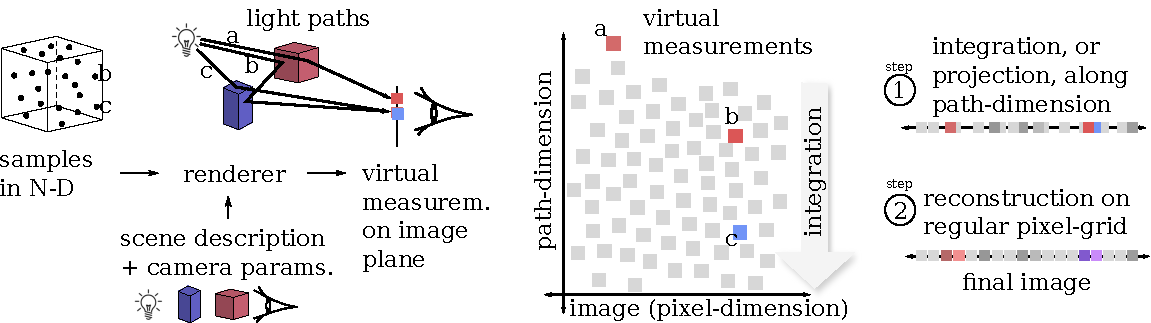
\includegraphics[width=\linewidth]{RenderHL.pdf}
 }
 \caption{\emph{The renderer implicitly maps samples from some high-dimensional space to light paths in a specified scene. The contributions of radiant light energy along these paths are recorded on the image plane as virtual measurements. Three light paths (a,b,c) are shown along with their canonical samples in the (hyper-) cube. The next two steps of rendering are integration along the path-dimension (step 1) followed by reconstruction on a regular grid (step 2). In this course, we focus on the impact of Fourier spectral properties of the canonical samples on the errors due to numerical integration.}}
 \label{fig:renderhl}
\end{figure}


\section{The interplay between reconstruction and integration}\index{Reconstruction and integration}
Images are typically represented and displayed on a regular grid. Rendering algorithms, however, may estimate virtual measurements at arbitrarily points on the sensor. We refer to the process of resampling the measurements \Ij{}\ on a regular grid as \textit{2D reconstruction}. Some rendering algorithms~\cite{Hachisuka:2008,Egan:2009,Soler:2009,Cov5D} partition the space of paths ($\Omega$ in equation~\ref{eq:measeq}) explicitly into dimensions that are dependent on the camera, such as exposure time and aperture, and those that depend on the scene. Since the sensor is two-dimensional, exposure time is one-dimensional and the aperture is two-dimensional, they estimate virtual measurements in a five-dimensional, camera-dependent space. This involves a reconstruction in 5D followed by a further projection (integration) down to the two-dimensional plane of the sensor. Such a partitioning is exploited for efficient rendering of camera-dependent blur effects resulting from relative motion between the camera and the scene or from defocus due to a finite (rather than infinitesemal) aperture.

\TBC

\section{The role of sampling}
There are two distinctly different applications of sampling in the rendering process (see figure~\ref{fig:renderhl}). One of them is for reconstruction, either in 2D or in 5D (as described above), and the other is for estimation of integration, which lies at the core of light transport (equation~\ref{eq:measeq}). Most rendering algorithms focus on the latter and perform reconstruction on a two-dimensional regular grid of pixels. Path-tracing, a popular rendering algorithm, proceeds by estimating the virtual image measurement at each pixel by averaging the values of the measurement contributions of a chosen set of paths through each pixel. Each path in the chosen set is obtained via a mapping from a sampling pattern (of appropriate dimensionality) to a set of rays in the scene. These sampling patterns may be stochastic (Monte Carlo sampling) or deterministic patterns that satisfy desirable criteria (Quasi-Monte Carlo). The statistics of the estimates of the virtual measurements yielded by these two broad classes of algorithms are strikingly different, as is the mathematical machinery used for their analyses.  

\TBC

\section{Sources and manifestation of error}\index{Error in rendering}
Error in the context of estimating global illumination~\cite{arvo1994framework} arises from three sources: inaccuracies in the  input data or simulation, errors due to discretization and computational errors such as loss of precision. In this course, we focus on the first two sources. The rendered image is represented on a discrete grid, while the distribution of the underlying light energy across the sensor is a continuous function. A major source of error stems from this discretization. The underlying continuous function is a high-dimensional integral at each point on the sensor (equation~\ref{eq:measeq}). Any sampling-based approach used to estimate this function results in an approximation whose measured deviation from the true function is known referred to as \textit{approximation error}. Typically this error manifests in rendered images as structured artifacts or noise. 
% Various metrics, such as L1 norms, L2 norms, PSNR, etc., are used to quantify approximation error.

\TBC 

%----------------------------------------------------------------------------------------
%	CHAPTER 2
%----------------------------------------------------------------------------------------
\chapterimage{ch2.pdf} % Chapter heading image
\chapter{Mathematical preliminaries}
% We review relevant mathematical concepts and introduce the notation adopted in this course.


\section{Random variables, expectation and variance}
For the purpose of this course, it will suffice to think of random variates simply as variables whose value is subject to chance. 
 For formal definitions of random variables and functions of random variables, we refer interested readers to introductory textbooks on probability or Monte Carlo simulation~\cite{robertc10}.
 We will restrict ourselves to continuous random variables, denoted using bold capital letters (\RV X, \yii,~etc.), that assume values in some domain \Dom. 
 The relative likelihood for continuous random variables to take on a given value is specified using a (normalized) probability density function (pdf) $\sdsym: \Dom \rightarrow \R$. We denote that \RV X\ is distributed according to \sdn\ by $\RV X \sim \sdn$. The probability that the random variable lies in a subdomain $\Domi{i} \subset \Dom$ is obtained as 
% \begin{equation}
  $\Prob(\RV X \in \Domi{i}) = \DefIntT{\Domi{i}}{}{\sdn}{x}.$
% \end{equation}

A function $\phi:\Dom\rightarrow\R$ evaluated at a location specified by a random variable, $\phi(\RV X)$, is also a random variable.
In this course, we are primarily concerned by the first two moments of random variables (specifically functions of random variables). The first moment, or ``average value'' of a random variable is captured by the mathematical concept of the \textit{expected value} of the random variable. We denote the expected value of \RV X\ as 
$ \Expf{\phi(\RV X)}{\sdsym}   \equiv \DefIntT{\Dom}{}{\phi(x)\;\sdsym(x)}{x}$. 

If the pdf has an expected value, the variance of the random variable is its second central moment which we denote
$\Varf{\phi(\RV X)}{\sdsym} \equiv \Expf{\phi^2(\RV X)}{\sdsym} - \Expf{\phi(\RV X)}{\sdsym}^2$. 
When \RV {X}\ is distributed uniformly within the domain (i.e.~\sdn\ is a constant), we drop the subscript and write the expectation as \Exp{\phi(\RV X)} and the variance as \Var{\phi(\RV X)}.

\TBC 

\section{Estimators}
Consider Monte Carlo estimation of the multidimensional integral $ I = \DefIntT{\Dom}{}{\ifn}{x}, \; \x\in\Dom $.A simple \emph{primary} MC estimator for $I$ is
$\estim{1}\equiv\ifsym(\RV X) , \;\RV X \in \Dom$. When \RV X\ is distributed
uniformly, the estimator is unbiased. That is, its expected value is the integral:$\Exp{\estim{1}}=\Ival$. The function \ifsym(\RV X)\ is itself a random variable with an arbitrary distribution and, typically, a large variance. A more practical MC estimator is obtained by averaging a fixed number of (say \N) primary estimates:  $\estim{\N} = \sum \ifni/\N, \; i=1,2,...,\N$. Such \emph{secondary estimators}  are known to be unbiased and approach Gaussian distributions as \N\ is increased, if the primary estimator has finite variance. 

\TBC 

\begin{table}[hbpt]%
\caption{\label{tab:notation}%
A summary of notation used in this course.\TBC}%
\setlength{\extrarowheight}{0.3cm}
\begin{tabular}{rl}%
    \toprule
    Symbol & Definition\\
    \midrule
    \ifn 	&  integrand \\
    $\w(x)$	&  sample weights\\
    \sdn 	&  sampling distribution (pdf) \\
    \estim{\N} 	&  estimate of $I$  using \N\ samples \\
%     \estim{is,\N} 	&  \N-sample importance sampling estimator\\
%     \estim{is,1} 	&  primary (1-sample) imp. samp. estimator\\
    \RV X, \RV Y, \xii, \yii & random variates \\
    $\PowerSpec{S}(\fv)$ &
	  Power spectrum of \sfn \\ %: $\PowerSpec{S}(\fv) = $
    $\sfn \Fdual \SF $&
          Fourier transform pair: integrand and its transform\\
    $\sfn \Fdual \SF $&
          Fourier transform pair: sampling function and its transform\\
    $\Exp{\phi(\RV X)}$ 		&
      Expectation: $\DefIntT{\Dom}{}{x\;\phi(x)}{x}$\\[-2pt]
    $\Var{\phi(\RV X)} $ 						&
      Variance : $\DefIntT{\Dom}{}{x\;\phi^2(x)}{x} -
      \DefIntT{\Dom}{}{x\;\phi(x)}{x}$\\
    $\Expf{\phi(\RV X)}{\sdsym} $ &
      Expectation with $ \RV X \sim \sdn$:
$\DefIntT{\Dom}{}{\phi(x)\;\sdsym(x)}{x}$\\[-2pt]
% $\Exp{\phi^2(\RV X)} - \Exp{\phi(\RV X)}^2$\\
    $\Varf{\phi(\RV X)}{\sdsym} $					&
Variance with $ \RV X \sim \sdn$:
  $\DefIntT{\Dom}{}{\phi^2(x)\sdn}{x} -
      (\DefIntT{\Dom}{}{\phi(x)\sdn}{x})^2$\\
\bottomrule
\end{tabular}
\end{table}

\section{The continuous Fourier transform}

The process of solving differential equations is simplified by projecting relevant functions onto a basis formed by eigenfunctions of the differential operator. The class of functions $x \rightarrow \MyExp{\imag \fvn x}$ forms a natural choice since $\frac {\mathrm{d}}{\mathrm{d}x} \MyExp{\imag \fvn x} = \imag \fvn . \MyExp{\imag \fvn x}$. The projection of a given function, $\ifsym: \Re \rightarrow \C$, results in a set of coefficients --- one coefficient corresponding to every function in the basis (so, per choice of \fvn). If the basis is chosen so that it contains continuous (real) values of \fv, the corresponding coefficients may be viewed as a function of \fv. $\IFsym: \Re\rightarrow\C$. Under certain conditions
\footnote{
We refer readers to textbooks on the subject~\cite{} for a mathematically rigorous treatment.
}
 the relationship between \ifn\ 
and its coefficients of projection \IFn\ can be written as 
\begin{eqnarray}
 \label{eq:FT} \IFn & = & \DefInt{-\infty}{\infty}{\ifn \; \MyExp{- \imag 2\pi \fv x}}{x}  \\
 \label{eq:IFT} \ifn & = & \DefInt{-\infty}{\infty}{\IFn \; \MyExp{ \imag 2\pi \fv x}}{\fv}.
\end{eqnarray}
The integral transforms in eq.~\ref{eq:FT} and eq.~\ref{eq:IFT} are known as the \textit{Fourier transform} and the \textit{inverse Fourier transform} respectively. Due to Euler's formula in complex analysis,  $\MyExp{\imag 2\pi \fv x} = \cos({2\pi\fvn x}) + \imag \sin({2\pi\fvn x})$, the projection of functions onto complex exponentials is equivalent to a projection onto sinusoids of frequencies given by $2\pi\fv$. For this reason, \fv\ is referred to as the \textit{frequency variable} and \IFn\ is said to be a representation of \ifn\ in the \textit{frequency domain}. We denote the Fourier transform pair using \ifn \Fdual \IFn. In summary, the continuous Fourier transform decomposes a function on the infinite (real) domain into a continuous sum (integral) of sinsuoids of continuous and unbounded set of frequencies. The set of continuous complex coefficients arising from this decomposition is called the \textit{Fourier spectrum} of the function. 

\section{Fourier series}
The projection of periodic functions onto complex exponentials leads to a special case. Consider a general periodic function \ipn T\ obtained by convolving a function \ifn\ with a Dirac comb \shaf{T} with period $T$. Since $\ipn T = \ifn  \conv \shaf T$, the Fourier transformed periodic function is a product $\IPn T = \IFn \SHAF T$ (due to the convolution theorem). Since \SHAF T\ is also a Dirac comb (with a period of $1/T$ in the frequency domain), the Fourier spectrum of \ipn T\ is only non-zero at the set of locations where \SHAF T\ is non-zero. Therefore, the Fourier spectrum of a continuous periodic function is non-zero at discrete (regular) frequencies.

The inverse Fourier transform of the periodic function can then be written as a summation:
\begin{eqnarray}
  \ipn T & = & \sum\limits_{n\in\Z}^{} c_n \; \MyExp{\imag 2\pi n x / T}.
\end{eqnarray}
The $c_n$, known as the \textit{Fourier series coefficients}, are obtained as 
\begin{eqnarray}
\label{eq:cn}  c_n & = & \frac 1 T \; \DefInt{x_0}{x_0+T}{\ifn \; \MyExp{- \imag 2\pi n x / T}}{x} \;\; = \;\; \frac {\IFsym (n/T)} T
\end{eqnarray}
where $x_0$ is any choice for $x$ so that \ifn\ is integrable within $[x_0, x_0+T]$. Typically the complex exponential in eq.~\ref{eq:cn} is expanded in terms of $\sin{}$ and $\cos{}$, leading to two sets of coefficients. This crucial observation, that even periodic functions with discontinuities may be expressed as the sum of an infinite set of harmonics was made by Joseph Fourier in his study of heat. It was subsequently rigorously proved by Fourier's prot\'eg\'e, Peter Dirichlet, who also outlined requirements for convergence of the Fourier series. Dirichlet's results formed the theoretical foundation which led to the derivation of the continuous Fourier transform. 


\section{Discrete time Fourier transform (DTFT)}
Recall that the Fourier transform of a periodic function results in a discrete spectrum. Conversely, the Fourier transform of a uniformly sampled continuous function results in a periodic Fourier spectrum. Consider the a discrete function obtained by sampling by a Dirac comb.~i.~e.~ the function is $\ifn . \shaf s$, where $s$ is the sampling period. The resulting Fourier spectrum (of the discrete function) will be the convolved spectrum, $\IFn \conv \SHAF s$, which is periodic (with a period of $1/s$).


\section{The Discrete Fourier transform (DFT)}
In practice, Fourier analysis is often performed on sampled functions that span a finite domain. In most cases, the discrete function is also assumed to be replaced by its periodic version with a period equal to the width of the domain. Combining the analysis for Fourier series and DTFT, we can write the input function as $\ipn{sT} = (\ifn . \shaf s) \conv \shaf T$. The Fourier transform of this discrete-time periodic function is $(\IFn \conv \SHAF s) . \SHAF T$ which is periodic (with a period of $1/s$) and discrete due to the frequency-domain sampling by \SHAF T.

Given data $f_n, \; n=0,1,...,N-1$, the $k^{th}$ ($k\in\Z$) coefficients of the DFT and IDFT are 
\begin{eqnarray}
 \label{eq:DFT}c_k &=& \quad \sum\limits_{n=0}^{N-1} f_n \; \left( \cos{(-2\pi k n/N)} + \imag \sin{(-2\pi k n/N)} \right) \;\; \mathrm{and}\\
 \label{eq:IDFT} f_n &=& \frac 1 N \sum\limits_{k=0}^{N-1} c_k \; \left( \cos{(-2\pi k n/N)} + \imag \sin{(-2\pi k n/N)} \right)
\end{eqnarray}
respectively. Due to periodicity, the domain of k is typically $[0,N-1]$. The DFT is a linear, invertible transformation $\mathcal{F}_{DFT}: \C \rightarrow \C$ that exhibits most properties of the continuous Fourier transform such as completeness and orthogonality. Also, important theorems such as the convolution theorem, shift theorem, Plancherel's and Parseval's theorems also have their equivalents in the context of the DFT. Na\"ive calculation of the $N$ coefficients $c_k$ requires $O(N^2)$ computation since each coefficient involves a summation over $N$ terms. Fast Fourier Transform (FFT) algorithms solve this with $O(N \log{N})$ computation.

\section{Power spectral density (PSD) and the periodogram}
The energy of a signal \ifn\ is generally considered to be the integral of the square of the signal (over its entire domain). Due to Parseval's theorem, this may also be expressed as the integral, over all frequencies, of the square (for real signals) of the Fourier transform of the signal. The integrand in this expression of power, $|\IFn|^2$, is referred to as the \textit{power spectrum} of \ifn. We denote the PSD of $f(x)$ as $\PowerSpec{f}(\fv)$, which represents the squared amplitude of the Fourier coefficients at the frequency \fv. 

Now consider a wide-sense stationary random processes, from which a single observation is made. The data from this observation may be subjected to Fourier analysis and the PSD of the observed data --- called a \textit{periodogram} --- may be considered as an estimate of the PSD of the generating process. Although the periodogram is not a very good estimate~\cite{}, it is convenient and hence popular~\cite{lagaeDutre}. 
% Look at Bartlett 55
% Need to clean up usage of periodogram and power spectrum
% cite http://www.dcs.warwick.ac.uk/~feng/teaching/PowerSpectrum.pdf
\TBC

%----------------------------------------------------------------------------------------
%	CHAPTER 3
%----------------------------------------------------------------------------------------
\chapterimage{ch3.pdf} % Chapter heading image
\chapter{Sampling for reconstruction}
The reconstruction problem entails approximating a function $\ifsym:\Dom\rightarrow\R$ as $\appr{\ifsym}(x_i), \; x_i\in\Dom, \;i=1,2,3,...,M$ given $\ifsym(y_i), \; y_i \in \Dom, \;j=1,2,3,...,\N$, where the sets of points $\{x_i\}$ and $\{y_j\}$ are mutually exclusive. If $\appr{\ifsym}(y_j) = \ifsym(y_j),\;\forall j$, the process is referred to as interpolation. This problem has received much attention in the signal processing literature~\cite[chapters~5~\&~6]{engineering2008handbook} as well as in the rendering community~\cite{Wold85,Cook:1986:SSC,mitchell87a,journals/cga/Blinn89a}. Such analyses have yielded effective reconstruction filters that are used in modern renderers, especially in low-dimensional domains such as the image plane.

Reconstruction is akin to nonlinear regression~\cite{GVK394929411}, a popular problem in the statistics (and more recently machine learning) literature, which offers effective solutions in high-dimensional settings when the approximand exhibits stationarity or accurate solutions for smooth and low-dimensional approximands. In rendering, the underlying functions represent a multitude of combinations (products, convolutions and sums) of a variety of non-stationary processes such as spatio-directional lighting, hard shadows, sharp reflections, textured materials, etc. The resulting discontinuities and variations in the radiant light energy (radiance function) across space-angle-time pose immense challenges which state of the art methods in non-linear regression are unable to cope with.

The reconstruction process generally consists of two steps. First, for any point $x$ in the domain, the influence of each of the $\ifsym(y_j)$ samples is specified using some \textit{weighting kernel} on the distance between $x$ and $y_i$ (typically Euclidean). Then, at each of the $x_i$, the approximate value is obtained by summing up the distance-weighted contributions of each of the $\ifsym(y_j)$. Depending on the choice of the kernel and the strategy for determining weights, the resulting methods are known by different names: Kernel Smoothers, Radial Basis Functions, Shepherd's method, etc.  

\section{Aliasing in reconstruction}
The general reconstruction process (above) may be written in terms of the underlying function (or signal). The samples, $\ifsym(y_i), \; y_i \in \Dom$, can be represented as the  product of the true (often unknown) function \ifn\ with a sampling function of the form $S(x) = \sum\limits_{j=1}^{\N} \updelta(x-y_j)$. 
If $K(r)$ represents the kernel weight at a distance of $r$, the continuous approximand and its Fourier dual are
\begin{equation} \label{eq:recons}
 \appr{\ifsym}(x) = \left(\ifn . S(x) \right) \conv K(x) \Fdual 
 \appr{\IFsym}(\fv) = \left(\IFn \conv \FTsym{S}(\fv)\right) . \FTsym{K}(\fv) 
\end{equation}
where \conv\ denotes convolution. That is, the effect of sampling can be seen in the Fourier domain as one of generating spurious replicas of \IFsym\, created due to the convolution with $\FTsym{S}$, which potentially hinders perfect reconstruction.   The kernel, on the other hand, can be viewed as a low-pass filter which suppresses replicated, or aliased, copies of the true function's spectrum at high frequencies. 

If \ifn\ contains frequencies less than $\fv_b$ (is band-limited), if the sampling spectrum does not contain frequencies lower than $2\fv_b$, and if the kernel is a low-pass filter suppressing frequencies above $\fv_b$, the resulting reconstruction will be perfect. If these conditions are not satisfied, the approximation will contain error. The first potential source of error is that \ifn\ is not bandlimited and hence, regardless of the sampling function, the low-pass effect of the kernel results in the loss of high-frequencies. The other main source of error is due to the sampling spectrum containing low frequencies, which results in a \FTsym{\appr{\ifsym}}\ that contains a superposition of \IFn\ with its aliased copies.

\section{Antialiasing}
The error introduced by aliasing either appears as coherent structure or as noise, depending on the choice of sampling spectrum. Sampling on a regular grid corresponds to multiplication with a Dirac-train or Shah function, whose Fourier spectrum remains a Shah function. If the samples are not sufficiently dense in the image plane, the resulting spectrum contains impulses at lower frequencies which cause aliasing in the form of regular structure that has been shown to be particularly unpleasant to our perceptual system. If the function being reconstructed is bandlimited, and in the absence of a sampling budget, the sampling rate may be increased to eliminate aliasing. However, if the function contains arbitrarily high frequencies, a simple strategy is to introduce randomness in the spectrum thereby transforming coherent artifacts into visual noise. This has shown to be less objectionable to our visual systems.

\TBC

\section{Halftoning}
Halftoning is the process of determining a sampling function $S(x)$ so that a kernel density estimate of the sampled function $\appr{\ifsym}(x) = \ifn.S(x)$ provides the best approximation to \ifn. It is a special case of reconstruction where the kernel is implicit and dependent on our visual systems. Halftoning methods strive to identify sampling functions for which the \textit{perceived} sampled function is as close to \ifn\ as possible. This may be achieved by varying the distributions of the samples, by weighting them or using a combination of both. Densely sampled regions of the sampled function are perceived to have darker tone. 

\TBC

\section{Antialiasing as integration}
Antialiasing is commonly viewed as an integration problem. The value to be assigned to a pixel is often estimated by averaging sampled values within a square around the pixel. That is, pixels are viewed as little squares and the values assigned to pixels are obtained by integrating the underlying function within their respective squares. On the contrary, if pixels are viewed as simply being points on the image plane~\cite{smith1995pixel}, this choice of integrating within the pixel appears to be an arbitrary choice. That is, it corresponds to performing reconstruction on the image plane exactly as in equation~\ref{eq:recons}, with $K(x)$ chosen to be a box with a width that is half the inter-pixel distance, followed by resampling of $\appr{\ifsym}(x)$ on a regular grid. Although this view of antialiasing is better than not performing antialiasing, it is well known that the box-filter is not the ideal choice. Modern renderers offer a variety of choices for the pixel reconstruction filter, since its choice is dependent on the rendering algorithm chosen and the corresponding sampling patterns used for estimating light energy arriving at the pixel~\cite[section~7.6]{Pharr:2010:PBR:1854996}.

\TBC
%----------------------------------------------------------------------------------------
%	CHAPTER 4
%----------------------------------------------------------------------------------------
\chapterimage{ch4.pdf} % Chapter heading image
\chapter{Estimating integrals}
It has long been known that the problem of numerical integration lies at the heart of rendering~\cite{Perlin89Course}. The main objective of rendering is to estimate the quantity of radiant light energy impinging on the various pixels (or cells) distributed on a virtual observer's camera (or eye). Current renderers perform this via physically-based simulation of light, following its intricate combinations of reflections within the scene. The virtual measurement \Ij {\xs} at a point \xs\  on the sensor~\cite[ch.8]{Veach:1998:RMC:927297} is
\begin{eqnarray} \label{eq:measeq}
 \Ij {\xs} & = & \DefInt{\Omega}{}{f_\xs(\pth)}{\mu(\pth)}
\end{eqnarray}
where the measurement contribution function, $f_\xs(\pth)$, is the importance-weighted radiance arriving at \xs\ along the path \pth\ and $\mu(\pth)$ is a measure on the space of all paths $\Omega$. The paths \pth\ span space as well as time and may be of arbitrarily high dimensionality. 

The exact nature of the integrand depends on the complexity and structure of the scene being rendered, along with detailed modelling of the constituent materials and shapes.  In general, the integrand is high-dimensional, discontinuous and costly to evaluate. Each evaluation of the integrand requires many rays to be traced within the environment, along with estimation of the radiant light energy along that path formed by linking the rays together. 
The rendering community strives to estimate such integrals with low error as well as low computational cost.


\section{Numerical integration via sampling}
Henceforth in this chapter, we abstract away the details about the integrand and domain of integration (equation~\ref{eq:measeq}) that is encountered in rendering. We study the integration problem in the canonical domain.  
Our goal is to analyze the of quality of numerical integration, within the interval $[0,\Tx]$, of a function $\ifsym: \R \mapsto \R^{+}$. 
% in terms of the Fourier spectrum of the underlying sampling strategy. 
For example, a \textit{primary} Monte Carlo estimator $\estim{1} = \ifsym(\xii)$ for the integral
\begin{equation} \label{eq:integcanonical}
I \equiv \frac 1 \Tx \DefInt{0}{\Tx}{\ifn }{\x}  
\end{equation}
is well known to be unbiased if the  single sample $\xii \in [0,\Tx] $ is drawn from a constant probability distribution function (pdf) within the domain $[0,\Tx]$.~i.e.~$\Exp{\estim{1}} = I$.
The corresponding secondary estimator, obtained by averaging \N\ primary estimates at different \xii\ has the same expected value. However, the averaging scales the variance down by a factor of $\N$.~i.e.~$\Var{\estim{\N}} = \Var{\estim{1}}/\N.$ 

\TBC
\begin{figure}
 \centering
 {
  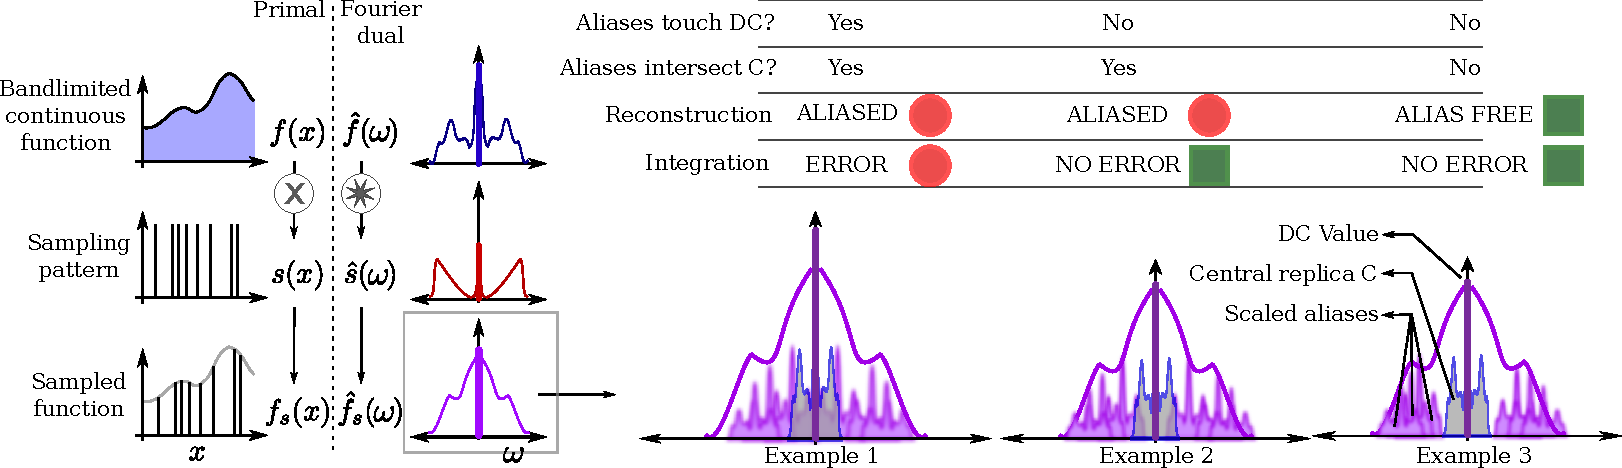
\includegraphics[width=\linewidth]{IntegRecons.pdf}
 }
 \caption{\emph{This figure highlights the difference in the analysis of sampling rates for error-free reconstruction vs numerical integration of a bandlimited function. Fewer samples (factor of 2 per dimension~\cite{Cov5D}) are sufficient for error-free numerical integration.}}
\end{figure}

\section{Error due to sampling: Convergence rate, consistency, bias and variance} 
Numerical integration methods like Monte Carlo are very powerful in approximating the underlying  multi-dimensional integrand using stochastically generated samples, but the overall process is highly prone to error. The nature of the error introduced depends on an intricate combination of three factors: the distribution of the sample locations; the weighting used to accumulate sampled contributions; and the arrangement (correlation) and structure of samples. The ``error'' of an estimator, which refers to its mean squared error (MSE), typically reduces as the number of samples is increased. The rate at which this reduction occurs is known as the estimator's \textit{convergence rate}. Estimators whose errors vanish in the limit are said to be \textit{consistent}.

The MSE of an estimator is comprised of two different types of error: One that is associated with the accuracy of the estimator, and another which describes the precision of the estimates. The former, which is the deviation of the expected value from the true (or desired) result is known as \textit{bias}. The latter, which quantifies the uncertainty of the estimator is known as \textit{variance}. The MSE is expressed as the sum of the squared bias and the variance.

Consistent estimators, whether biased or unbiased, are desirable for image synthesis. Although objectionable image artifacts may be produced by the use of na\"ively-designed biased estimators (say using regular sampling), in many cases connsistent and biased estimators are used to reduce noise as well as to improve convergence rates~\cite{Keller:2012:AMCCourse}. 

% Bias is defined as the value by which the numerically integrated value deviates from the ground truth value. In the Fourier domain, bias can be represented as an expected value of the error~\cite{Subr:2013:FAS}. Another form of error is variance which is manifested in the form of noise during image synthesis. Variance represents the uncertainty in the primary Monte Carlo estimates. 

%\subsection{Variance (uncertainty of estimates)} 
%Another form of error is variance which is manifested in the form of noise during image synthesis. %Variance represents the uncertainty in the primary Monte Carlo estimates. 

%\GURPRIT{
%Unless I am missing something I don't see why uncertainty refers to Variance. For me uncertainty is a relative concept. For example, 
%the variance of a kernel in the primal and the fourier domain cannot be predicted simultaneously at a given frequency. Reducing variance in one domain would increase variance in the other, which is what 
%uncertainty is all about. }
%\KARTIC{Random variables introduce uncertainty. Variance is one form of the quantification of uncertainty. If you are estimating Variance, then you can talk about uncertainty of the variance estimates. I like to pose the process of quantifying error in the estimates as a form of uncertainty propagation (\url{https://en.wikipedia.org/wiki/Propagation_of_uncertainty}). That is, if we know the uncertainty in the sampling patterns, can we estimate uncertainty in the final estimates?}

%!TEX root = main.tex
%
% Start with sampling patterns 
%
%
\subsection{Manifestation of error in rendering}
For a given scene configuration (hence fixed integrand), the error in the rendered image is primarily dependent on the choice of sampling strategy. To a lesser extent, the error also depends on the algorithm used for rendering (path-tracing, Metropolis light transport, etc.). The motivation behind using stochastic sampling over regular samples was related to human perception. The bias caused by using regularly placed samples is considered more objectionable~\cite{} to our visual systems than its appearance as noise that is distributed across all frequencies (see fig.~XX for an example). 

Consider an image rendered using path tracing with 64 samples per pixel. Each pixel in the final image can be viewed as a single instance of a secondary estimator, of the integral corresponding to that pixel, using 64 samples. In theory, the variance of each of these estimates can only be observed by rendering multiple images with 64 samples per pixel. In practice, even though the integrand at each pixel is different, the radiance varies smoothly over many parts of the image. As a result, if estimators for pixels in these smooth regions have high variance, their disagreement on particular instances of the estimate (in the rendered image) leads to a noisy appearance. The larger the disagreement of estimates in neighboring pixels in smooth regions, the noisier the image will appear. In other words, an estimator with a higher variance will lead to a noisier image.

The manifestation of bias is less intuitive. Typically, estimators with a structured bias --- such as one that uses a regular sampling pattern --- produce banded visual artifacts. In some cases, bias leads to artifacts that are inconsistent with our expectation of realism.~e.~g.~bright patches at points where contact shadows are expected. Bias may also lead to incorrect estimates where the error is not visually perceivable. Such estimators are desirable, particularly if they can simultaneously improve the visual noise The solution to the inveterate problem of striking a reasonable compromise between bias and variance, for efficiency, depends on the nature of the scene, choice of sampling strategy, number of samples, etc. 

The reduction of error, for a given sampling strategy, might be achieved by increasing the number of samples. So, in the above example, rendering with 128 or 256 samples per pixel will reduce noise. 
% The rapidity with which variance diminshes, as the number of samples is increased, is called the \textit{convergence rate} of the estimator. 
Some estimators (jittered sampling, QMC sampling) converge faster than others. Even for a fixed sampling strategy, primary and secondary estimators have different distributions and hence different statistics. Secondary estimators approach being Gaussian-distributed, as the number of the fixed samples used is increased. Choosing the ``best'' estimator depends on the application. For high-quality, offline rendering the estimator of choice will be the one with the quickest convergence. On the other hand, for applications with a time-budget, the estimator with the lowest error for the given budget of samples must be chosen.

\begin{figure}
\begin{tabular}{c c c}
\multicolumn{3}{c}{samples on a regular grid (biased and consistent)}\\
%   \begin{sideways} regular (biased) \end{sideways} & 
  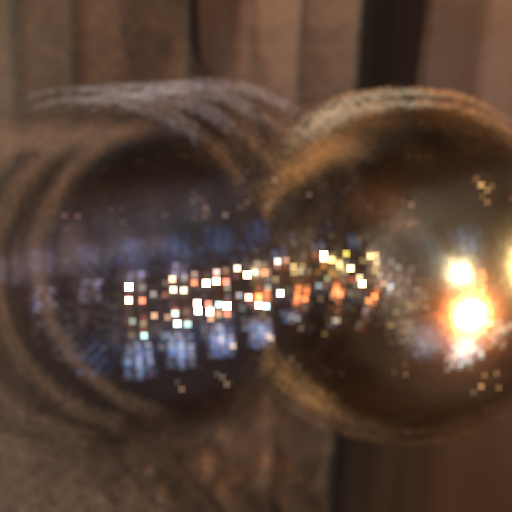
\includegraphics[width=.3\linewidth]{../PBRTOut/pngs/testmb_ball.scene_GRID_2_Samps_iter_1_1_uj.exr.png}&
  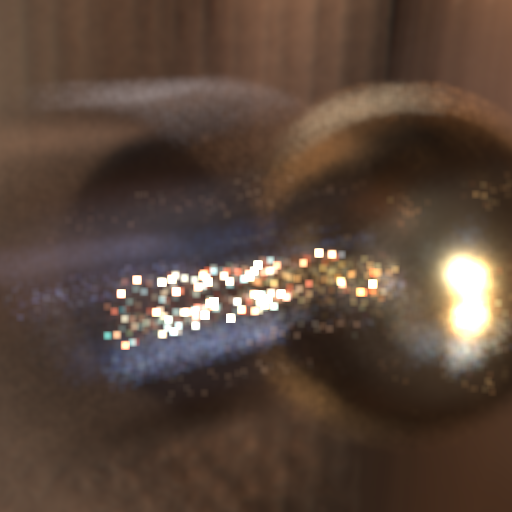
\includegraphics[width=.3\linewidth]{../PBRTOut/pngs/testmb_ball.scene_GRID_4_Samps_iter_1_1_uj.exr.png}&
  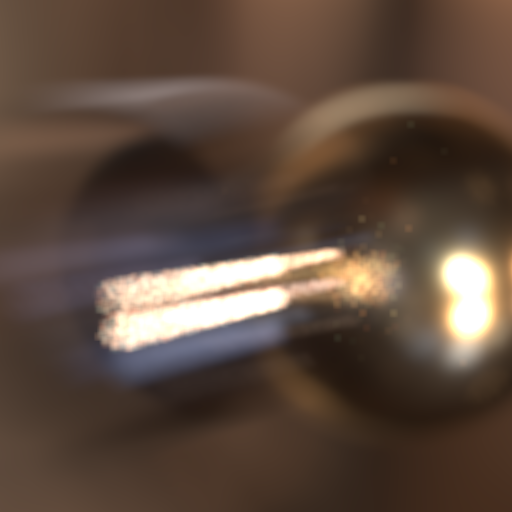
\includegraphics[width=.3\linewidth]{../PBRTOut/pngs/testmb_ball.scene_GRID_64_Samps_iter_1_1_uj.exr.png}\\
  \hline
\multicolumn{3}{c}{low-discrepancy sampler (biased and consistent)}\\
%     \begin{sideways} low discrepancy (biased) \end{sideways} &
  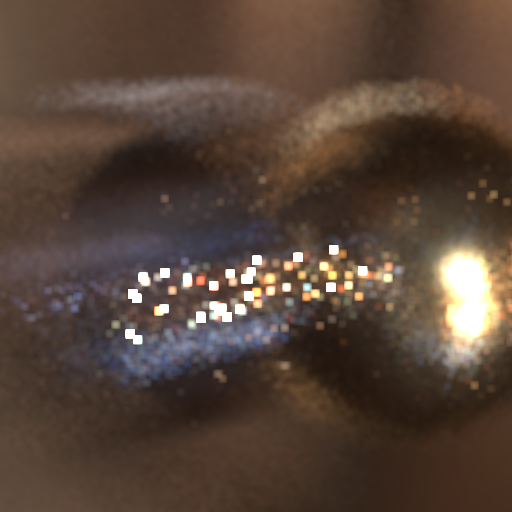
\includegraphics[width=.3\linewidth]{../PBRTOut/pngs/testmb_ball.scene_LD_4_Samps_iter_1__uj.exr.png}&
  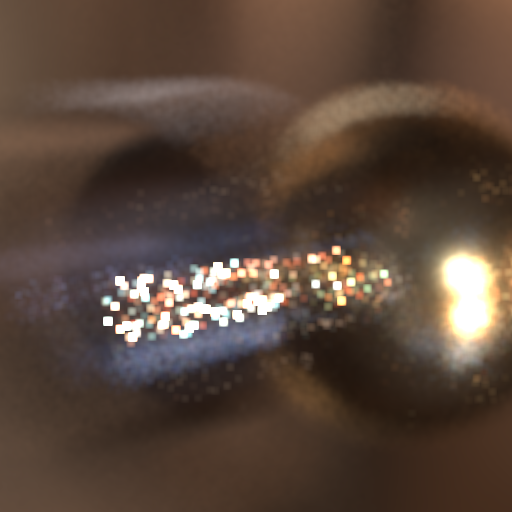
\includegraphics[width=.3\linewidth]{../PBRTOut/pngs/testmb_ball.scene_LD_16_Samps_iter_1__uj.exr.png}&
  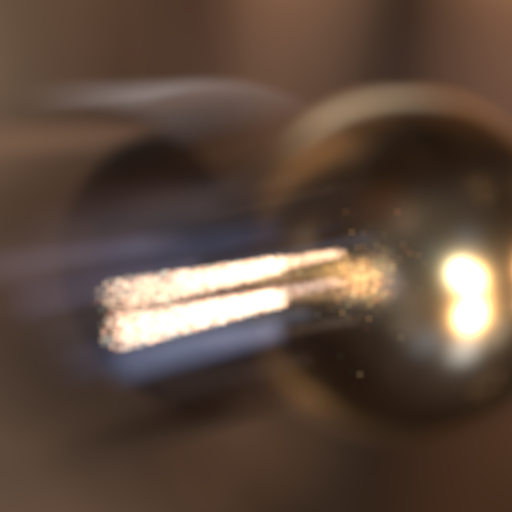
\includegraphics[width=.3\linewidth]{../PBRTOut/pngs/testmb_ball.scene_LD_4096_Samps_iter_1__uj.exr.png}\\
\hline
\multicolumn{3}{c}{random sampling (unbiased and consistent)}\\
%     \begin{sideways} random (unbiased) \end{sideways} &
  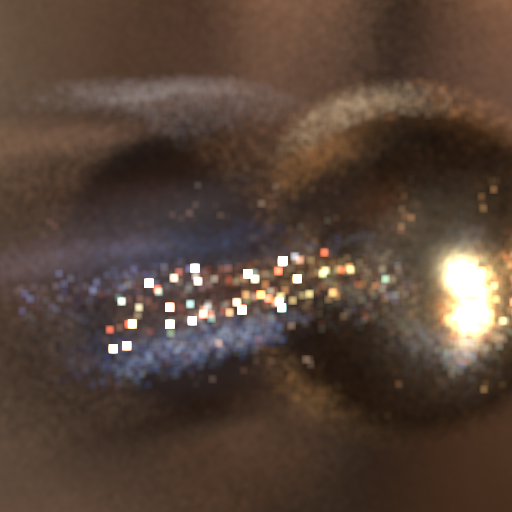
\includegraphics[width=.3\linewidth]{../PBRTOut/pngs/testmb_ball.scene_RAND_4_Samps_iter_1__uj.exr.png}&
  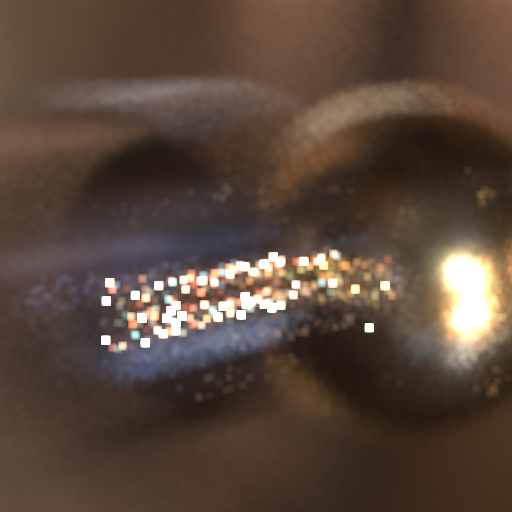
\includegraphics[width=.3\linewidth]{../PBRTOut/pngs/testmb_ball.scene_RAND_16_Samps_iter_1__uj.exr.png}&
  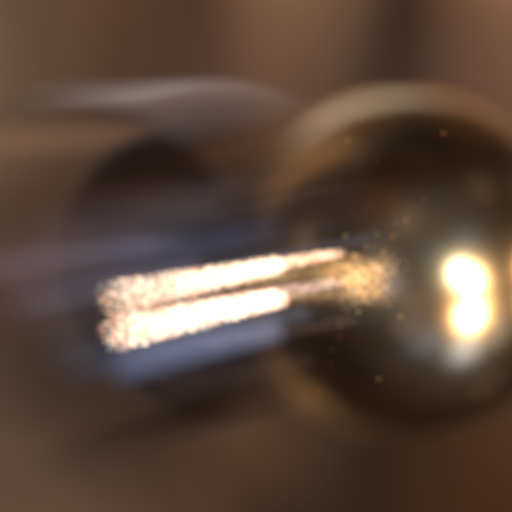
\includegraphics[width=.3\linewidth]{../PBRTOut/pngs/testmb_ball.scene_RAND_4096_Samps_iter_1__uj.exr.png} \\
   4 samples per pixel (spp)& 16 spp& 4096 spp \\
\end{tabular} 
\label{fig:errorrender}
\caption{A comparison of rendered results obtained using 3 sampling strategies (rows) for various sampling counts (columns). The images depict two shiny balls: A golden ball that is out of focus and a mirrored ball  that is moving rapidly through the plane in focus. All strategies lead to consistent estimators, therefore the images in the third column are virtually indistinguishable. The na\"ive, biased strategy of sampling on a regular grid leads to objectionable visual artifacts. A more sophisticated approach --- low-discrepancy sampling (middle row) --- although biased, not only eliminates the regular artifacts but also exhibits improved noise characteristics (for example in the background region, using 16 samples) compared to unbiased estimates obtained using random sampling (bottom row). }
\end{figure}




\subsection{Homogenization}
The analytical characterization of both, bias as well as variance, across a general set of sampling strategies is challenging. 
% Analysing both bias and variance at the same time in Monte Carlo integration can be challenging. 
 However, focusing on unbiased estimators makes it possible to express error in the form of variance only. To apply this analysis to a wide variety of estimators, it would be beneficial to first be able to transform them into unbiased estimators, albeit by introducing extra variance. 
 One way to mitigate the bias of an estimator is by ensuring that the sampling spectrum only contains energy at the DC~\cite{Subr:2013:FAS}. Inspired by the process of generating unbiased estimators from randomly jittering a regular grid~\cite{Ramamoorthi:2012}, Pilleboue et al~\cite{Pilleboue:2015:VAM} shifted each realization of the samples by uniformly random amounts. They termed this process \textit{homogenization}. In the point processes literature homogenization is also known as \emph{stationary point processes} for which the average number of points per some unit of extent such as length, area, volume, or time, is constant depending on the underlying mathematical space.

%\subsection{Consistency}
%\TBC

% \subsection{Consistency and Convergence}
% Sampling strategies for which error goes down with the increase in number of samples are considered consistent. Although, reducing variance in Monte Carlo estimators have been given paramount importance in the past, it is also worth while to investigate the convergence rate, which represents the rate at which error goes down with the increase in the number of samples. 

\section{Monte Carlo integration in the Fourier domain}
Monte Carlo sampling can be represented as an inner product of the integrand \ifn\ and a random sampling pattern \sfn\ which is composed of a sum of impulses (delta functions) normalized by the number of impulses (see Sec.~\ref{sec:sfn}). Since inner products are preserved under Fourier Transforms, the na\"ive estimator  can be expressed in the frequency domain as 
\begin{equation}
  \estim{\N} \quad = \quad \DefInt{\Dom}{}{\ifn \sfn}{x} \quad = \quad 
  \DefInt{\Omega}{}{\SF \; \IFsym^*(\fv) }{\fv}, 
\end{equation}
where $\IFsym^*(\fv)$ is the complex conjugate of the Fourier transformed integrand. Since the goal is to represent the spectrum of a stochastic process, which is generally not integrable over the infinite domain, it is important that the integral is restricted to the finite domain \Dom. The definite integral can either be viewed as a multiplication by a box of the appropriate dimensions~\cite{Subr:2013:FAS} or as a portion of a periodic function on a toroidal domain~\cite{Pilleboue:2015:VAM}. The former leads to a 'virtual' integrand which subsumes the convolution by a \sinc (the Fourier transformed box), while the latter leads to a discrete Fourier spectrum (see Sec.~\ref{sec:PFT}). This reformulation of numerical integration provides a fresh perspective on the analysis of error. The derivation of MSE~\cite{FredoTR}, convergence~\cite{Pilleboue:2015:VAM}, bias and variance~\cite{Subr:2013:FAS} in terms of the statistics of the Fourier spectra of the sampling function and the integrand provide valuable insight into the design of adaptive sampling strategies.


%\section{Assessing sampling patterns based on their spectra}
%
%!TEX root = main.tex
%
% Start with sampling patterns 
%
%
\section{Assessing sampling patterns based on their spectra}

\subsection{Qualitative assessment using periodograms}
Following the seminal work by Robert Ulichney on \emph{blue noise} dithering~\cite{Ulichney:87:halftoning}, sampling patterns with minimal energy in the low frequency zone of their power spectra are believed to be preferable, for applications such as stippling and numerical integration. Tools such as the \emph{periodogram} and its radially-averaged profile were introduced to the graphics community about three decades ago, and were primarily used for qualitative comparisons of sampling patterns. 
% Ulichney also proposed to use \emph{radially-averaged} power spectra, as a means of explicitly visualizing 
% which can be mathematically written as:
% %
% \begin{align}
% \RadialPowerSpec{\Sampling}(\RadialFreq) = \int_{\FreqVar = \RadialFreq} \PowerSpec{\Sampling}(\FreqVar) \Diff \FreqVar \,.
% \end{align}
%
%Periodograms does help in investigating low frequency zone region of sampling power spectra but it is not always possible to get a precise behaviour of periodograms for various sampling patterns like jitter and Poisson Disk. This is where radially averaged power spectra comes handy. By performing radial averaging of sampling power spectra we can get a closer and better look at the low frequency as well as the mid to high frequency regions of the sampling power spectra.
These tools have been used to compare the qualities of blue noise sampling patterns generated using various algorithms, and have been extended for comparisons between spatially-varying sampling distributions~\cite{Wei:2011:DDA}. 

\subsection{Quantifying error using the statistics of sampling spectra}
More recently, the focus has been on quantification of estimation error in the Fourier domain. That is, the error of an estimator (e.g.~\estim{1} for $I$ in equation~{eq:integcanonical}) has been expressed in terms of the Fourier spectra of the integrand and sampling function. 
% Monte Carlo integration has been only recently unfolded in a step by step manner starting from Durand~\cite{durand2011frequency}, Subr and Kautz~\cite{Subr:2013:FAS}, and then by 
% shortcite
Durand~\cite{durand2011frequency} derived mean-squared error (MSE) as the inner product of the spectral densities of the integrand and sampling function, 
\begin{equation} \label{eq:durand11}
   \Exp{(I-\estim{1})^2} = \DefInt{\Omega}{}{|\IFn|^2 \; \Exp{|\SF|^2}}{\fv},
\end{equation}
and verified that the convergence rate of the MSE of \estim{\N}\ is indeed $1/\N$. Following this work, it was shown~\cite{Subr:2013:FAS} that the bias and variance of \estim{1}\ may be expressed separately in terms of the spectra. They derived
\begin{eqnarray}
  \Exp{I-\estim{1}} &=& I - \DefInt{\Omega}{}{\Exp{\SF} \; \IFn }{\fv}, \quad \mathrm{and} \\
    \Var{\estim{1}} &\leq& \DefInt{\Omega}{}{\Var{\SF} \; |\IFn|^2}{\fv}
\end{eqnarray}
as the expressions for bias and variance respectively.~i.e.~An estimator's bias is dependant on the relationship between the expected Fourier spectrum of the sampling pattern and the integrand's spectrum. The second equation, shows that the estimator's variance is bounded by the variance present in the sampling spectrum relative to the spectral density of the integrand. Subsequently, these results were collated and the expression for the variance was reformulated~\cite{Pilleboue:2015:VAM} for homogenized (unbiased) Monte Carlo estimators as
%
\begin{equation} \label{eq:pillebouevar}
\Var{\estim{1}} 
= \DefInt{\Omega}{}{\Exp{|\SF|^2}\;|\IFn|^2}{\fv} 
= \DefInt{\Omega}{} {\Exp{\PowerSpec{\SFsym}(\fv)} \PowerSpec{\ifsym}(\fv)} {\fv} 
\end{equation}
which is identical to Durand's derivation of MSE (equation~\ref{eq:durand11}) for a general (possibly biased) \GURPRIT{I think Durand derived the variance for only random (white noise) samples, as he mentioned. Pilleboue obtained the same variance formulation but it was generalised to all samplers, thanks to the homogenization property} estimator. However, the homogenized perspective yields important insights and results on the convergence rate of estimators. \GURPRIT{I don't understand this statement, are you saying thanks to homogenization the convergence rates can be obtained ? }
%

\subsection{Quantifying convergence using periodograms}
The primary advantage of studying the variance of the homogenized (equation~\ref{eq:pillebouevar}) estimator was that it allowed an analysis of the convergence rate of estimators in terms of their power spectra. In addition, the homogenization process provides an elegant means of quantitatively comparing errors due to random (Monte Carlo) sampling patterns with deterministic (quasi Monte Carlo) patterns. 
\GURPRIT{We should be careful while making statements about the QMC methods. Although we can use the homogenization property for any sampling pattern we do not give any insights on how our Fourier analysis would yield convergence rates for QMC methods. This is tricky because QMC methods like Sobol can give different power spectra depending on the number of samples used. Pilleboue et al's method 
do not handle these cases.
}
\TBC
%

\section{Analysis beyond the canonical domain}
In rendering, Monte Carlo integration is not restricted to the Euclidean domain. For example, direct and global illumination methods involve integration over a visible  hemisphere of directions at the surface hit points, and over the sphere of directions in the presence of participating media within the scene. In this section we discuss a variety of such contexts. In particular, we focus on a closed form formulation for variance in the ( hemi-)spherical domain. 

%!TEX root = ./../main.tex
%
% Start with sampling patterns 
%
%
\subsection{Spherical domain}
On the sphere, the most commonly used tool for spectral analysis is spherical harmonics
(SH)~\cite{Groemer1996}, which is analogous to Fourier analysis on a (hyper-) plane. While the bases for Fourier analysis are chosen to be Eigenfunctions of the derivative operator on the plane, SH bases are chosen to be Eigenfunctions of the rotation invariant differential operator (Laplacian) on the sphere and are
%
\begin{equation}
\label{eq:SH}
Y_l^m(\theta,\phi) \equiv {\sqrt{(2-\delta_{0m})\frac{(2l+1)}{\Lebesgue{\SphericalDom{2}}}\frac{(l-m)!}{(l+m)!}}} \, P_l^m(\cos\theta) \, \exp({im\phi})\,.
\end{equation}
%
Here, $\delta_{ij}$ is the Kronecker delta function, $\Lebesgue{\SphericalDom{2}}=4\pi$, is the Lebesgue measure of a unit 
sphere, $Y_l^m(\theta,\phi)$ is the spherical harmonic basis
function of degree $l$ and order $m$ and $P_l^m(x)$ denotes  the \emph{asssociated Legendre
Polynomials}, for $x \in [-1,1]$. SH $(Y_l^m)$ are orthonormal basis functions such that  any integrable function
$\DummyIntegrand$ on $\SphericalDom{2}$ can be decomposed into SH components.
 as:
 %
\begin{align}
\label{eq:SHDecomposition}
\DummyIntegrand(\SpaceVar) = \sum_{l=0}^{\infty} \sum_{m=-l}^{l}  \SPH{\DummyIntegrand}(l,m) \, Y_l^m(\SpaceVar)\,,
\end{align}
%
where $\SPH{\DummyIntegrand}(l,m)$ are the (complex) spectral coefficients of $\DummyIntegrand(\SpaceVar)$. 
It can be easily shown that:
%
\begin{equation}
%\label{eq:SHParsevalF}
\int_{\SphericalDom{2}} \Norm{\DummyIntegrand(\SpaceVar)} \Diff\omega = \sum_{l=0}^{\infty} \sum_{m=-l}^{l} \Norm{\SPH{\DummyIntegrand}(l,m)}\,.
\end{equation}

which is the Parseval's theorem on the sphere. Analogously,
the inner product between any two arbitrary functions, $\DummyIntegrand(\SpaceVar)$ and
$\Integrand(\SpaceVar)$ defined over a unit sphere, is related to their corresponding spectral coefficients by:
%
\begin{equation}
%\label{eq:SHParsevalGF}
\int_{\SphericalDom{2}} \DummyIntegrand(\SpaceVar) \, \mathrm{\overline{\Integrand}}(\SpaceVar) \, \Diff\SpaceVar =
\sum_{l=0}^{\infty} \sum_{m=-l}^{l}\, \SPH{\DummyIntegrand}(l,m)\cdot\overline{\SPH{\Integrand}(l,m)}\,,
\end{equation}
%
where $\SPH{\DummyIntegrand}(l,m)=\langle\DummyIntegrand,Y_l^m\rangle$ is the $(l,m)$-th spherical harmonic coefficients of $\DummyIntegrand(\SpaceVar)$. The angular mean power spectrum at a frequency band $l$ is defined as the average energy distributed over different $m$ for a given $l$, as follows:
%
\begin{equation}
%\label{eq:angular_power}
\RadialPowerSpec{\DummyIntegrand}(l) \EqDef \frac{1}{2l+1} \sum_{m=-l}^{l} \left\|\SPH{\DummyIntegrand}(l,m)\right\|^2\,.
\end{equation}
%
The \emph{mean} angular power spectrum $\RadialPowerSpec{\DummyIntegrand}(l)$ is invariant 
under a rotation of the coordinate system (\cite{Kaula1967,lowes1974spatial}), as they contain a sum over all orders $m$. 
A spherical harmonic power spectrum can be defined with or without the averaging factor. In our formulation, 
we prefer to work with the average power per degree, or power spectral density, $\RadialPowerSpec{\DummyIntegrand}(l)$, as 
this ensures that the spectral coefficients of a spherical Dirac delta function are constant and independent of degree $l$  (\cite{hipkin2001statistics}). 

%
Based on this background, variance expression for Monte Carlo integration can be derived~\cite{Pilleboue:2015:VAM} in the spherical domain as:
%
\begin{align}
\label{eq:sphere_var_finale}
\Variance{\RvMCE} = \frac{\Lebesgue{\SphericalDom{2}}}{N} \sum_{l=0}^{\infty}\, (2l+1) \Exp{\PowerSpec{\RvSampling}(l)} \RadialPowerSpec{\Integrand}(l)
\end{align}
%
which gives the final expression for the variance in terms of the angular mean power spectra of both the sampling pattern 
$\RvSampling$ and the integrand $\Integrand$. 


%!TEX root = main.tex
%
% Start with sampling patterns 
%
%
\subsection{Other domains}

Recently, there has been interest in performing image synthesis by sampling in the gradient domain \cite{}. The path-tracing problem is reformulated to cover a multi-dimensional space spanning across paths and pixels. Rather than to estimate radiance at each pixel these methods estimate the gradients, in the subspace of pixels, of radiance. Finally, the image is reconstructed from the estimated gradients. The primary benefit of applying the gradient operator is that it attenuates the low-frequency content of the integrand. While jittered sampling reduces error by attenuating low-frequencies in the sampling pattern, gradient domain path tracing operates by reducing the low-frequency content of the integrand.  Although the gradient operator amplifies the energy at higher frequencies, it has been observed to remain within practical range at the Nyquist rate.

The spectral analysis of error due to stochastic sampling makes assumptions about the sampling strategy as well as the sampling domain. For extensions to domains with complex topology, or when non-uniform sampling is used, it is possible that other mathematical tools may be required. For example, Wei and Wang \cite{} proposed a formulation equivalent to Fourier analysis, but based on the distribution of the differentials of sampling locations. The use of this \textit{Differential Domain Analysis} permits the comparison of sampling strategies with different distributions.~e.~g.~two instances of the same sampling strategy, but with different target sampling densities, can be identified to have similar spectral properties. The advantages of the analysis are that it can be performed on general domains, and for non-uniform sampling. However, its invariance to distributions makes it less suitable for the analysis of error in integration. 


  
%
% Differential domain analysis
%

%
%
%


% %!TEX root = main.tex
%
% Start with sampling patterns 
%
%
\subsection{Gradient domain}


%----------------------------------------------------------------------------------------
%	CHAPTER 5
%----------------------------------------------------------------------------------------
\chapterimage{ch5.pdf} % Chapter heading image
\chapter{Popular sampling patterns} \label{ch:stateoftheart}
In this chapter, we will describe sampling strategies that are popularly used in modern renderers. For each of these, we provide insight on its error, explain the contexts where its behavior is best and/or worst and also comment on its expected convergence rate using its homogenized periodogram. For simplicity we will primarily discuss these sampling routines in the context of generating locations within a canonical unit square interval in 2D, and briefly explain how each routine generalizes to higher dimensions. Example slides for this topic are included (chapter~\ref{ch:exslides}).

\TBC

\section{Classical}
\subsection{Independent random sampling}
Purely independent random sampling is the most basic form of sampling pattern. When uniformly sampling a 2D square domain, the $x$ and $y$ coordinates of each point are computed from independently drawn uniform pseudo-random numbers $\xi \in [0,1)$. New sample points are generated without regard to the previously generated sample points. Figure~\ref{fig:independent-points} shows an illustration of 64 and 256 independent random samples in a unit square.

One benefit of this approach is that the sampling routine is trivially \textit{progressive}: we can continually add new samples without needing to know how many total sample points we will be generating. It is also trivial to generate samples in arbitrary dimensions by simply drawing a canonical random number $\xi$ for each dimension of a sample point. Unfortunately, however, since samples are drawn completely independently, the resulting sampling patterns many contain many samples which fall in close proximity while large regions of the sampling domain receive no samples.

Independent random sampling leads to the most basic form of Monte Carlo integration. The variance of a Monte Carlo estimator using independent random samples has a convergence rate of $\mathcal{O}(N^{-1})$. This result can be easily derived from the definitions of expected value and variance, but it can likewise be derived in the frequency domain from the periodogram of the sampling pattern. An important characteristic of this convergence rate is that (in contrast to deterministic quadrature techniques) the dimensionality of the integration problem does not appear in the expression for the convergence rate. Monte Carlo integration using independent random samples therefore does not suffer from the so-called ``curve of dimensionality''. This is one of the reasons why Monte Carlo techniques are so attractive for high-dimensional integration problems like the rendering of global illumination. Unfortunately, this convergence rate also means that error will always go down relatively slowly: we need four times as many samples to reduce the error by a factor of two.

Due to these limitations, many more sophisticated sampling techniques have been developed over the years which relax the assumption of independence in the hopes of reducing variance or improving convergence rate.

\subsection{Stratified/Jittered sampling}
Stratified sampling divides the integration domain into a number of disjoint regions (a.k.a ``strata'' or ``cells''), and places one or more independent random samples within each region. Jittered sampling, introduced to graphics by Cook and colleagues~\cite{Cook:1986:SSC}, is a restricted form of stratified sampling where the strata are of equal size with each receiving exactly one sample. Jittered sampling of a 2D unit square involves dividing the square into a grid of $N = M\times M$ square cells, and placing a single sample randomly positioned inside each cell. For 2D, this process would result in $N^2$ samples. Figure~\ref{fig:jittered-points} shows an illustration of $8\times8 =64$ and $16\times16 = 256$ jittered sample points in a unit square.

Jittered sampling considerably reduces the likelihood that many samples will fall within close proximity, and, since each stratum is guaranteed one sample, also places a strict upper bound on the size of any region void of any samples. These two properties considerably improve how well evenly distributed the sample points are compared to independent random sampling. Unfortunately, this improvement comes at the cost of some inconvenience. Jittered sampling is not progressive, so we cannot continually add more samples, and we must know the total number of samples before constructing the point set. Furthermore, the total number of samples is only set indirectly through the number of subdivisions along each dimension. With the same number of subdivisions along each dimension, the total number of samples has to be a perfect square in 2D, a perfect cube in 3D, etc. This can be cumbersome, and becomes increasingly so as the dimensionality of the point set grows. Setting the total number of samples with fine granularity becomes increasing difficult, e.g. dividing each dimension of a five-dimensional domain into two cells results in $2^5 = 32 samples$ and increasing the divisions to three per dimension already increases the sample count to $3^5 = 243$. While it is possible to set an different number of subdivisions along each dimension to obtain finer granularity, it is not easy to determine these values automatically or optimally for a particular integration problem.

It can be shown that jittered sampling cannot increase the variance of a Monte Carlo estimator compared to using independent random samples. In fact, it can often reduce variance considerably. Moreover, analysis of the periodogram reveals that jittered sampling has can result in asymptotically better convergence rates of XXX and YYY.

\subsection{Uniform jittered sampling}
Uniform jittered sampling is a further restriction of jittered sampling where the random location of a point within its stratum is the same across the entire point set. In other words, a single jitter is applied to all samples of a regular uniform pattern (as opposed to jittering each stratum's sample independently as in jittered/stratified sampling). For the 2D unit square, any single realization of a uniform jittered sampling pattern is simply a randomly shifted rectangular grid pattern. Figure~\ref{fig:uniform-jittered-points} shows two independent realizations of 256 uniform jittered points.

Uniform jitter sampling can be beneficial for some low-dimensional problems in rendering. For instance, Pauly et al.~\cite{pauly00metropolis} used uniform jittered sampling for performing the one-dimensional line integral of radiance along each camera ray, and Ramamoorthi and colleagues~\cite{Ramamoorthi:2012} analyzed the error of uniform jittered sampling for integrating visibility from area light sources.


\subsection{Uncorrelated Jitter, N-Rooks, and Latin hypercube sampling}
To overcome the issue of generating jittered sample points in high dimensions, Cook et al.~\cite{Cook:1984:DRT} proposed to randomly combine jittered sample sets over subspaces of the full domain. For instance, to generate sample distributions for a nine dimensional space, we could separately partitioning four two-dimensional subspaces (e.g. pixel area, camera lens area, reflection direction, and shadow ray direction) as well as one one-dimensional subspace (time) and then combine the subspace dimensions at random. He called this technique uncorrelated jittering.

In 2D, generating $N$ samples would entail creating two separate 1D jittered point sets $X$ and $Y$ with $N$ samples each, and then using the samples in $X$ as the $x$-coordinate of each 2D point, and couple each $x$ with a $y$ from $Y$ in randomly permuted order. Another way to view this is that we must divide the 2D domain into $N$ rows and $N$ columns, and ensuring that example one 2D sample falls within any row or column. Shirley~\cite{Shirley91-DQMSD} called this idea $N$-Rooks sampling since the sample positions correspond to the arrangement of rooks on an $N\times N$ chessboard where none of the rooks can capture another in a single move. Figure~\ref{fig:jittered-points} shows an illustration of N-Rooks sampling patterns with $64$ and $256$ points in a unit square.

Combining $D$ randomly permuted 1D jittered samples in this way for arbitrary dimension $D$ is called Latin hypercube sampling. Like jittered sampling, this sampling approach is not progress as we need to know the total number of samples in advance. However, we can easily use an arbitrary number of samples, and no longer have to deal with the difficulty of specifying a $N = M^D$ samples for a $D$ dimensional domain.

Jittered sampling and Latin-hypercube sampling are related, but offer different stratification guarantees, and therefore have different variance reduction behavior. As an illustrative example, a 2D jittered sampling pattern with $N$ points will ensure that few samples can clump together in 2D, but as many as $\sqrt{N}$ samples may project to exactly the same location along either of the two axes (in other words, the projections actually correspond to $\sqrt{N}$ strata with $\sqrt{N}$ points in each stratum). On the other hand, a 2D Latin-hypercube sampling pattern with $N$ points provides less guarantees of clumping reduction in 2D, but ensures that along either of the axis projections each of the $N$ sample points falls into a different stratum. Latin-hypercube sampling can lead to better variance and convergence if the integrand does not depend strongly on some of the dimensions. In the extreme, where the integrand depends only on the $x$ coordinate, but not on $y$, Latin-hypercube sampling would provide better stratification of the relevant dimensions than jittered sampling.

\subsection{Multi-Jittered sampling}
Chiu et al.~\cite{chiu94multi} introduce multi-jittered sampling, which effectively enforces the stratification guarantees of jittered sampling and N-rooks sampling simultaneously: for $N=M\times M$ points in 2D we generate exactly one sample in each of the $M\times M$ strata, but also guarantee that there is exactly one sample in each of the $N$ rows and $N$ columns (projected strata along the coordinate axes). Figure~\ref{fig:jittered-points} shows an illustration of $8\times8 = 64$ and $16\times16 = 256$ multi-jittered sample points in a unit square.

\section{Quasi-Monte Carlo}
\subsection{Halton sequence}
\TBC
\subsection{Hammersley sequence}
\TBC

%!TEX root = main.tex
%
\section{Blue noise}
Any sampling pattern with Blue noise characteristics is suppose to be well distributed within the spatial domain without containing any regular structures. The term Blue noise was coined by Ulichney~\cite{Ulichney:87:halftoning}, 
who investivated a radially averaged power spectra of various sampling patterns. 
He advocated three important features for an ideal radial power spectrum;  
First, its peak should be at the principal frequency. % for that gray level.  
Second, the principal frequency marks a sharp transition level below which little or no energy exists. 
And finally, the uncorrelated high-frequency fluctuations are characterized by high-frequency white noise. Poisson Disk sampling pattern (shown in~\RefFig{powspec-radialmean-bluenoise}) closely resembles the above features in the low frequency zone.

%Yellot~\cite{Ylt83} studied the distribution of cones in an extrafoveal region of the eye of  a 
%rhesus monkey, which has a photoreceptor distribution similar to that in the humam eye. Yellot took 
%the optical Fourier transform of this distribution, which had characteristics of a \emph{Poisson Disk distribution}. 
%Motivated from the work by Yellot, Cook~\cite{Cook:1986:SSC} performed a 
%careful Fourier analysis of white noise, Poisson Disk and jittered sampling patterns. 
%He advocated the use of sampling patterns that lacks low frequency content. 
%Although, Cook in his theoretical analysis mentioned that the Fourier transform of Poisson Disk has 
%no low frequency content, Dipp\'{e} and Wold~\cite{Wold85} have correctly shown an offset in the low frequency zone of the spectrum of Poisson Disk using the \emph{flat field response noise spectrum}. 
%
%Even though Dippe and Wold, Cook and Mitchell~\cite{mitchell87a} clearly indicated the importance of no low frequency content in the 
%sampling patterns' Fourier spectra, the characteristics of an optimal sampling Fourier spectrum was still missing. Ulichney~\cite{Ulichney:87:halftoning}, in 1987, was the first to provide qualitative 
%characterization of a good sampling pattern, which he called \emph{Blue Noise}.
%
%
%The nature of the spectral distribution property of various types of noise is mainly described by color 
%names. The most common example is \emph{white noise}, so named because its power spectrum is 
%flat across all frequencies with equal energy distributed in all frequency bands, 
%much like the visible frequencies in the white light. \emph{Pink noise} has 
%the power spectrum such that the power spectral density is inversly proportional to the frequency. 
%Green noise, as its name suggests, consists of primarily mid-range frequencies. 
%Robert Ulichney~\cite{Ulichney:87:halftoning} also mentioned the curious case of \emph{brown noise}, named for the spectrum associated 
%with the Brownian motion~\cite{gardner1978white}. He introduced \emph{blue noise}, the high 
%frequency complement of the pink noise. Pink noise occurs very frequently in nature and thus is used 
%for physical simulation and biological distribution.
%
%\paragraph{Characteristics of Blue noise} 
%Ulichney performed a careful study of rectangular and hexagonal regular grid patterns to improve the 
%quality of digital halftones. He estimated the power spectrum of various grid patterns using the 
%Bartlett's method~\cite{bar64b}
%%cite{Bartlett:ZAMM1979}
%of averaging periodograms. He mentioned that a 
%desirable attribute of a well-produced halftone of a gray level is \emph{radial symmetry}. Therefore, 
%he investivated a radially averaged power spectra of various patterns. 
%Ulichney advocated three important features for an ideal radial power spectrum;  
%First, its peak should be at the principal frequency. % for that gray level.  
%Second, the principal frequency marks a sharp transition level below which little or no energy exists. 
%And finally, the uncorrelated high-frequency fluctuations are characterized by high-frequency white noise. 
%%In~\RefFig{ulichney-blue-noise}(b), taken from Ulichney's article, all these three regions are marked. 
%The radial power spectrum with above featurs is called the \emph{blue noise} power spectrum. 
%In the following subsections, we discuss various methods used to generate sampling patterns 
%with blue noise characteristics.

%\GURPRIT{
%I think the we can cover different classes of samplers if we can simply rename the subsections of this 
%section to the following: \\
%- Dart throwing based methods \\
%- Relaxation based methods \\
%- Tiling based methods 
%}
%\KARTIC{I've modified CCVT to Relaxation-based. However, I think Poisson-disk sampling is the general idea for which dart-based methods are used (rather than the other way around), so I've kept the first subsection PDisk}
%
%\GURPRIT{This is correct but we can also generate Poisson disk sampling using relaxation based methods 
%and/or tile based methods (Kopf et al.2006, Lagae and Dutre 2008). I was actually proposing to separate the generation process of sampling patterns. Dart throwing is one way of generating samples, which by 
%default give Poisson disk patterns. 
%}
\subsection{Poisson-disk sampling}
Poisson Disk sampling patterns can be generated by simply assigning a disk with minimum radius to each sample point and allowing new samples to get placed only outside the disk radii of existing samples. Cook~\cite{Cook:1986:SSC} proposed the first \emph{dart throwing} 
algorithm for generating Poisson Disk distributed point sets. 
Random samples are continually tested and only those that satisfy the minimum
distance constraint relative to samples already in the distribution
are accepted.

%As Ripley~\cite{Ripley77} mentioned, several point processes could be referred to as 
%``Poisson-disk'', but by strict definition, a true Poisson-disk process is realized by generating complete 
%patterns with Poisson statistics until one is found that meets the minimum-distance constraint. 
%Cook~\cite{Cook:1986:SSC} proposed the first \emph{dart throwing} 
%algorithm for generating Poisson Disk distributed point sets. 
%Random samples are continually tested and only those that satisfy the minimum
%distance constraint relative to samples already in the distribution
%are accepted.

For many years, dart-throwing was the only available method for
accurate Poisson-disk sampling. Its inefficiency led to the development
of approximate Poisson Disk sampling algorithms. For a more comprehensive summary of Poisson 
sampling methods developed in early years 
%developed till the year 2008, 
we refer the interested readers to the survey by Lagae and Dutre~\cite{journals/cgf/LagaeD08}.

\subsection{Relaxation-based methods}

There are many \emph{relaxation} based methods for the generation of blue noise sample 
distributions. 
%The early algorithms proposed were inspired from the traditional artistic technique of 
%stippling, which involves placing small dots of ink onto paper such that their density give the 
%impression of tone. The artist tightly controls the relative placement of the stipples on the paper to 
%produce even tones and avoid artifacts, leading to long creation times for the drawings. 
Lloyd~\cite{Lloyd.82} 
which is a powerful and flexible iterative method, is commonly used to enhance the spectral properties of 
existing distributions of points or similar entities. However, the results from Lloyd’s method are 
satisfactory only to a limited extent. First, if the method is not stopped at a suitable iteration step, the 
resulting point distributions will develop regularity artifacts. A reliable universal termination criterion to 
prevent this behavior is unknown. Second, the adaptation to given heterogenous density functions is suboptimal, requiring additional application-dependent optimizations to improve the 
results.

Balzer and colleagues~\cite{Balzer:2009:CPD:1531326.1531392} present a variant of Lloyd’s method, termed capacity constrained Voronoi 
tessellation (CCVT), which reliably converges towards distributions that exhibit no regularity artifacts and precisely adapt 
to given density functions. Like Lloyd’s 
method it can be used to optimize arbitrary input point sets to increase their spectral properties while avoiding its 
drawbacks. They apply the so called capacity constraint that enforces each point in a distribution to have the same 
capacity. Intuitively, the capacity can be understood as the area of the point’s corresponding Voronoi region weighted with 
the given density function. By demanding that each point’s capacity is the same, Balzer et al. ensure that each point 
obtains equal importance in the resulting distribution. This is a direct approach to generating uniform 
distributions, whereas Lloyd’s method achieves such distributions only indirectly by relocating the sites into the 
corresponding centroids.

\subsection{Tiling-based methods}

There are some tile-based approaches that can be used to generate blue noise samples 
Tile-based methods overcome the computational complexity of  
\emph{dart-throwing} and/or \emph{relaxation} based approaches in generating blue noise sampling patterns. In computer graphics community, two tile-based approaches are well known: First approach uses a set of precomputed tiles~\cite{Cohen:2003,Kopf:2006:RWT}, with each tile composed of multiple samples, and later use these tiles, in a sophisticated way, to pave the sampling domain. Second approach employed tiles with \emph{one sample per tile}~\cite{Ostromoukhov:2004:FHI,Ostromoukhov:2007:SP:1275808.1276475,Wachtel:2014:FTA} and uses some relaxation-based schemes, with look-up tables, to improve the over all quality of samples. 
Although many blue noise sample generation algorithms exist, none of them are easily extendable to higher dimensions $(> 3)$.
%\subsection{Discussion}

%Recently~\cite{Pilleboue:2015:VAM}, it has been shown that the low frequency region of the
%radial power spectrum (of a given sampling pattern) plays a crucial role in deciding the overall variance convergence rates of sampling 
%patterns used for Monte Carlo integration. Since blue noise sampling patterns contains almost no radial 
%energy in the low frequency region, they are of great interest for future research to obtain fast results in 
%rendering problems. Surprisingly, Poisson Disk samples have shown the convergence rate of $\BigO{N^{-1}}$ which is the same as given by purely random samples. This can be explained by looking at the low frequency region in the radial power spectrum of Poisson Disk samples (\RefFig{powspec-radialmean-bluenoise}) which is not zero.
%The importance of the shape of the radial mean power spectrum in the  low frequency region demands  methods and algorithms that could eventually allow sample generation directly from a target Fourier spectrum. Although many blue noise sample generation algorithms exist, none of them are easily extendable to higher dimensions $(>5)$.

%
%!TEX root = ../main.tex
%
%
\begin{figure}[t!]
\centering
\footnotesize
\begin{tabular}{@{}c@{\;}c@{\;}c@{\;}c@{}}
& Samples & Power spectrum & Radial mean \\
%
%=====================
%
\rotatebox{90}{\qquad\quad Random} & 
\begin{tikzpicture}
  \node[anchor=south west,inner sep=0] (image) at (0,0)
  {
    \pdfliteral{ 1 w}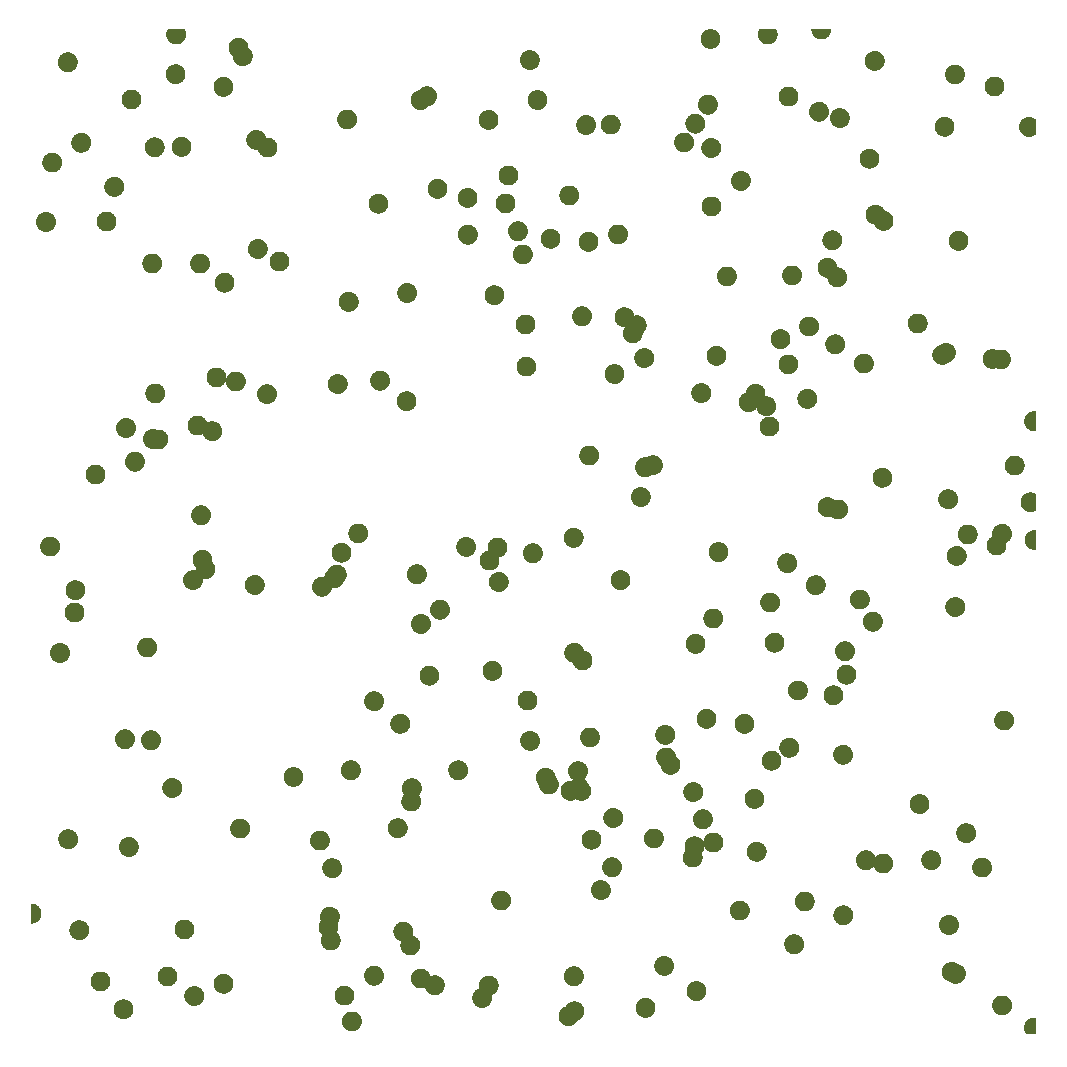
\includegraphics[width=0.2\columnwidth,page=1]{pointset/points-random-n256.pdf}
  };

  \begin{scope}[x={(image.south east)},y={(image.north west)}]
  \draw[black,thick] (0,0) rectangle (1,1);
  \end{scope}
\end{tikzpicture} 
&
\begin{tikzpicture}
  \node[anchor=south west,inner sep=0] (image) at (0,0)
  {
    \pdfliteral{ 1 w}
\includegraphics[width=0.2\columnwidth,page=1]{power-spectra/powerspectrum-random-n4096.png}
  };

  \begin{scope}[x={(image.south east)},y={(image.north west)}]
  \draw[black,thick] (0,0) rectangle (1,1);
  \end{scope}
\end{tikzpicture}
&
\begin{tikzpicture}
  \node[anchor=south west,inner sep=0] (image) at (0,0)
  {
    \pdfliteral{ 1 w}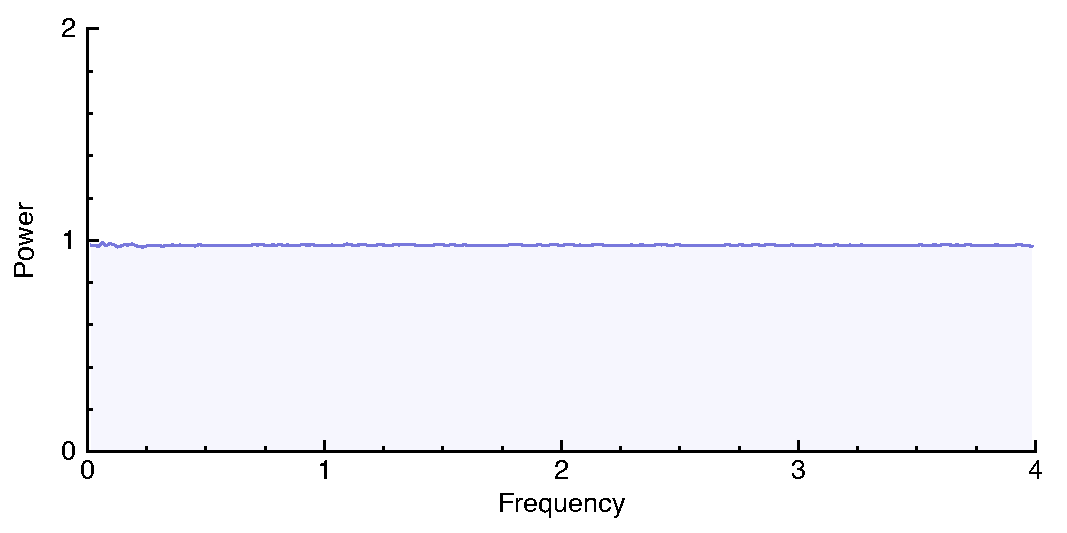
\includegraphics[width=0.4\columnwidth,page=1]{power-spectra/radial-mean-random-n4096.pdf}
  };

  \begin{scope}[x={(image.south east)},y={(image.north west)}]
  \draw[black,thick] (0,0) rectangle (1,1);
  \end{scope}
\end{tikzpicture}\\
%
%=====================
%
\rotatebox{90}{\qquad\quad Jitter} & 
\begin{tikzpicture}
  \node[anchor=south west,inner sep=0] (image) at (0,0)
  {
    \pdfliteral{ 1 w}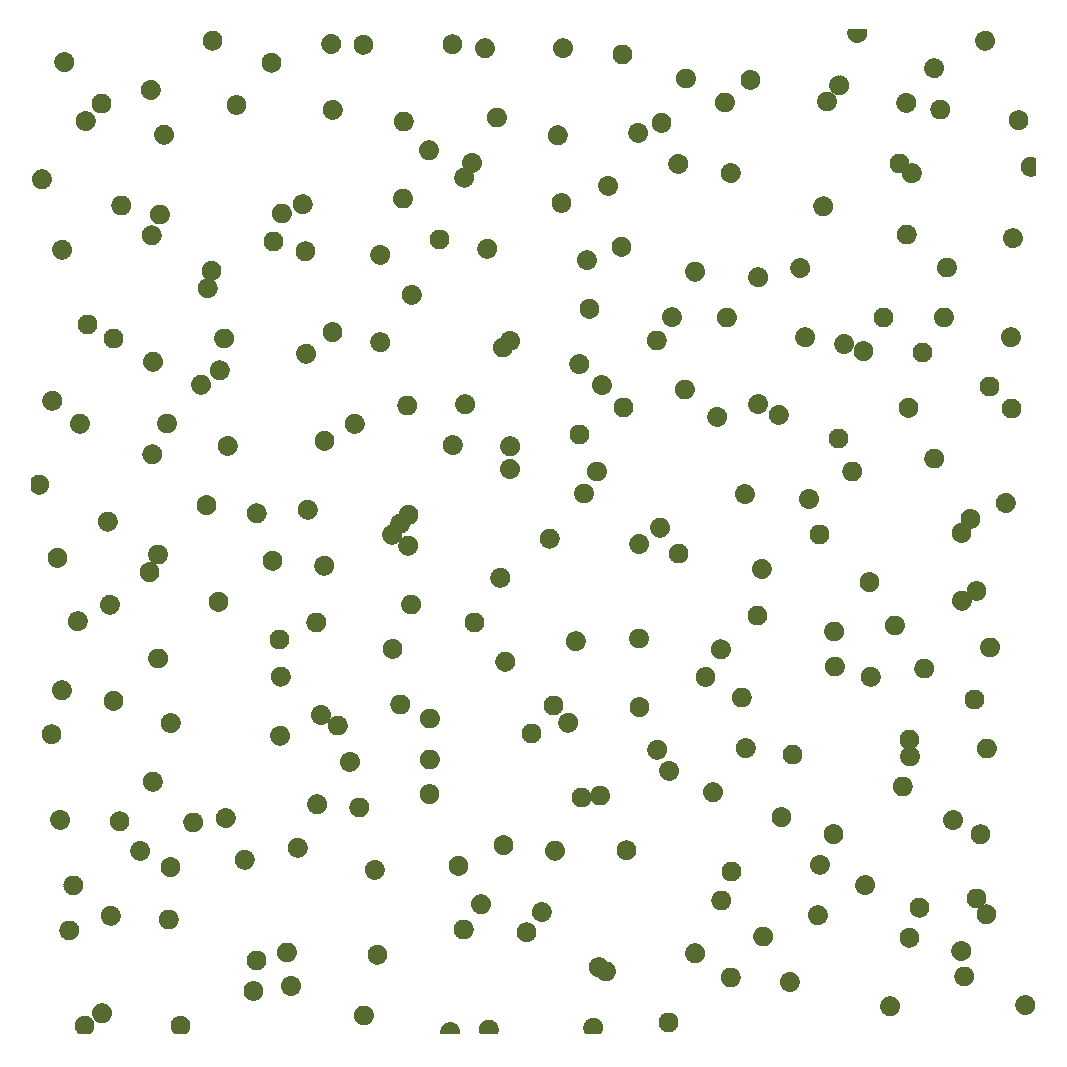
\includegraphics[width=0.2\columnwidth,page=1]{pointset/points-jitter-n256.pdf}
  };

  \begin{scope}[x={(image.south east)},y={(image.north west)}]
  \draw[black,thick] (0,0) rectangle (1,1);
  \end{scope}
\end{tikzpicture} 
&
\begin{tikzpicture}
  \node[anchor=south west,inner sep=0] (image) at (0,0)
  {
    \pdfliteral{ 1 w}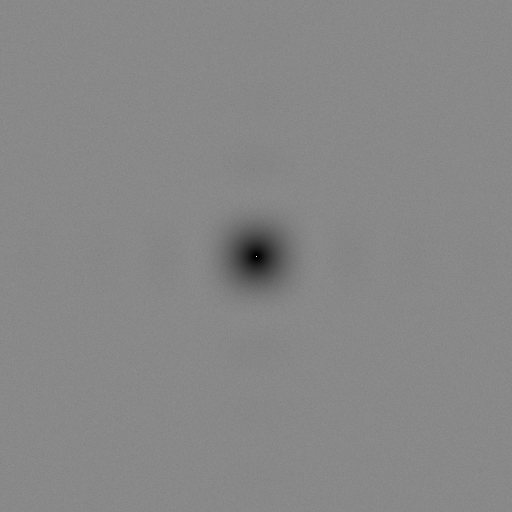
\includegraphics[width=0.2\columnwidth,page=1]{power-spectra/powerspectrum-jitter-n4096.png}
};

  \begin{scope}[x={(image.south east)},y={(image.north west)}]
  \draw[black,thick] (0,0) rectangle (1,1);
  \end{scope}
\end{tikzpicture}
&
\begin{tikzpicture}
  \node[anchor=south west,inner sep=0] (image) at (0,0)
  {
    \pdfliteral{ 1 w}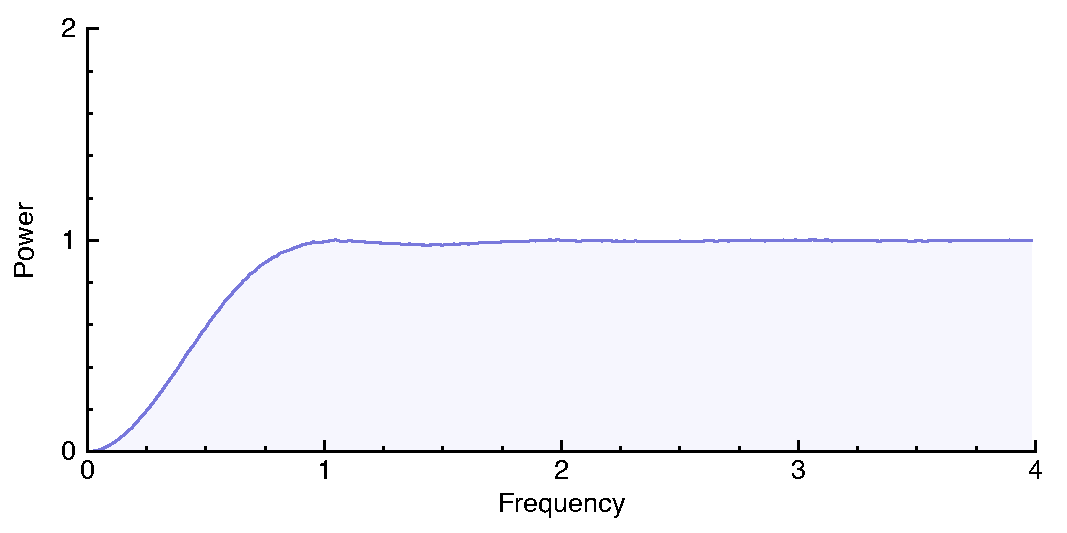
\includegraphics[width=0.4\columnwidth,page=1]{power-spectra/radial-mean-jitter-n4096.pdf}
  };

  \begin{scope}[x={(image.south east)},y={(image.north west)}]
  \draw[black,thick] (0,0) rectangle (1,1);
  \end{scope}
\end{tikzpicture}\\
%
%=====================
%
\rotatebox{90}{\quad\quad Multi-jitter} & 
\begin{tikzpicture}
  \node[anchor=south west,inner sep=0] (image) at (0,0)
  {
    \pdfliteral{ 1 w}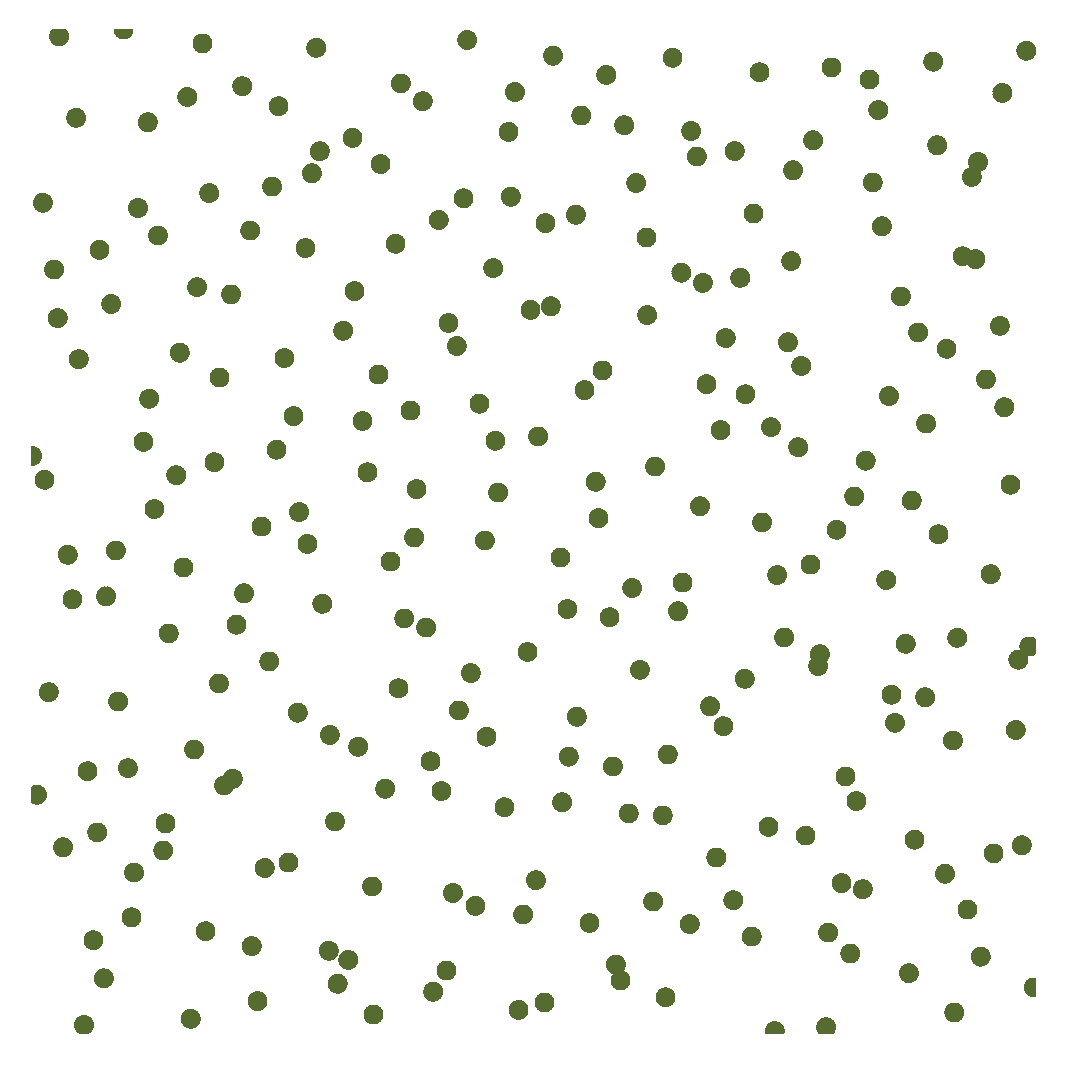
\includegraphics[width=0.2\columnwidth,page=1]{pointset/points-multijitter-n256.pdf}
  };

  \begin{scope}[x={(image.south east)},y={(image.north west)}]
  \draw[black,thick] (0,0) rectangle (1,1);
  \end{scope}
\end{tikzpicture} 
&
\begin{tikzpicture}
  \node[anchor=south west,inner sep=0] (image) at (0,0)
  {
    \pdfliteral{ 1 w}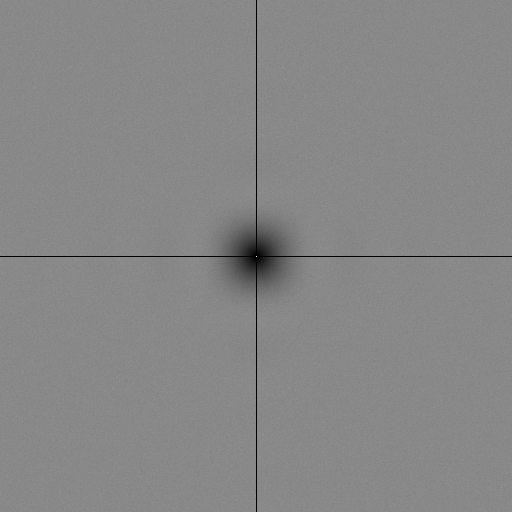
\includegraphics[width=0.2\columnwidth,page=1]{power-spectra/powerspectrum-multijitter-n4096.png}
  };

  \begin{scope}[x={(image.south east)},y={(image.north west)}]
  \draw[black,thick] (0,0) rectangle (1,1);
  \end{scope}
\end{tikzpicture}
&
\begin{tikzpicture}
  \node[anchor=south west,inner sep=0] (image) at (0,0)
  {
    \pdfliteral{ 1 w}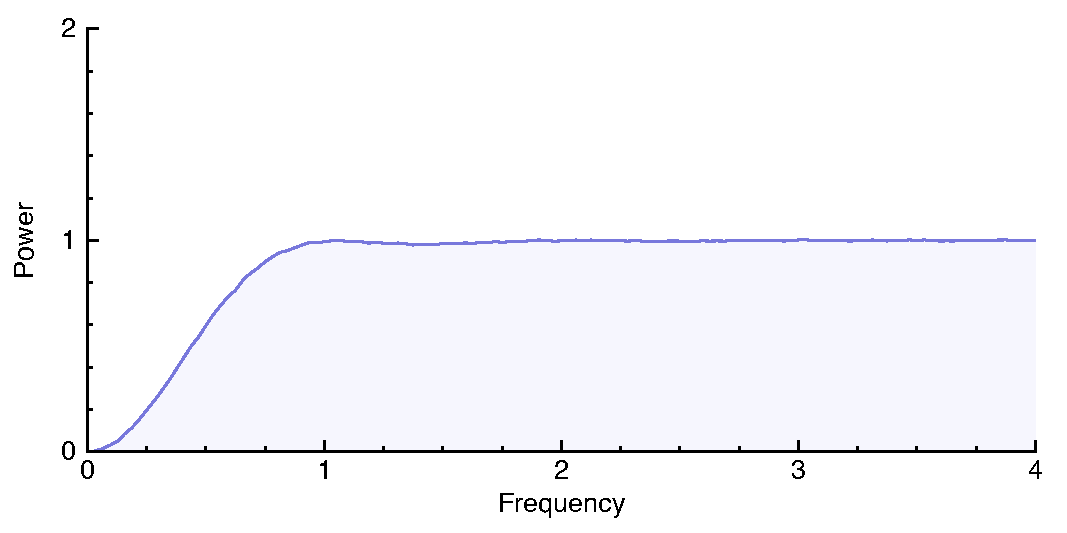
\includegraphics[width=0.4\columnwidth,page=1]{power-spectra/radial-mean-multijitter-n1024.pdf}
  };

  \begin{scope}[x={(image.south east)},y={(image.north west)}]
  \draw[black,thick] (0,0) rectangle (1,1);
  \end{scope}
\end{tikzpicture}\\
%
%=====================
%
\rotatebox{90}{\qquad\quad N-rooks} & 
\begin{tikzpicture}
  \node[anchor=south west,inner sep=0] (image) at (0,0)
  {
    \pdfliteral{ 1 w}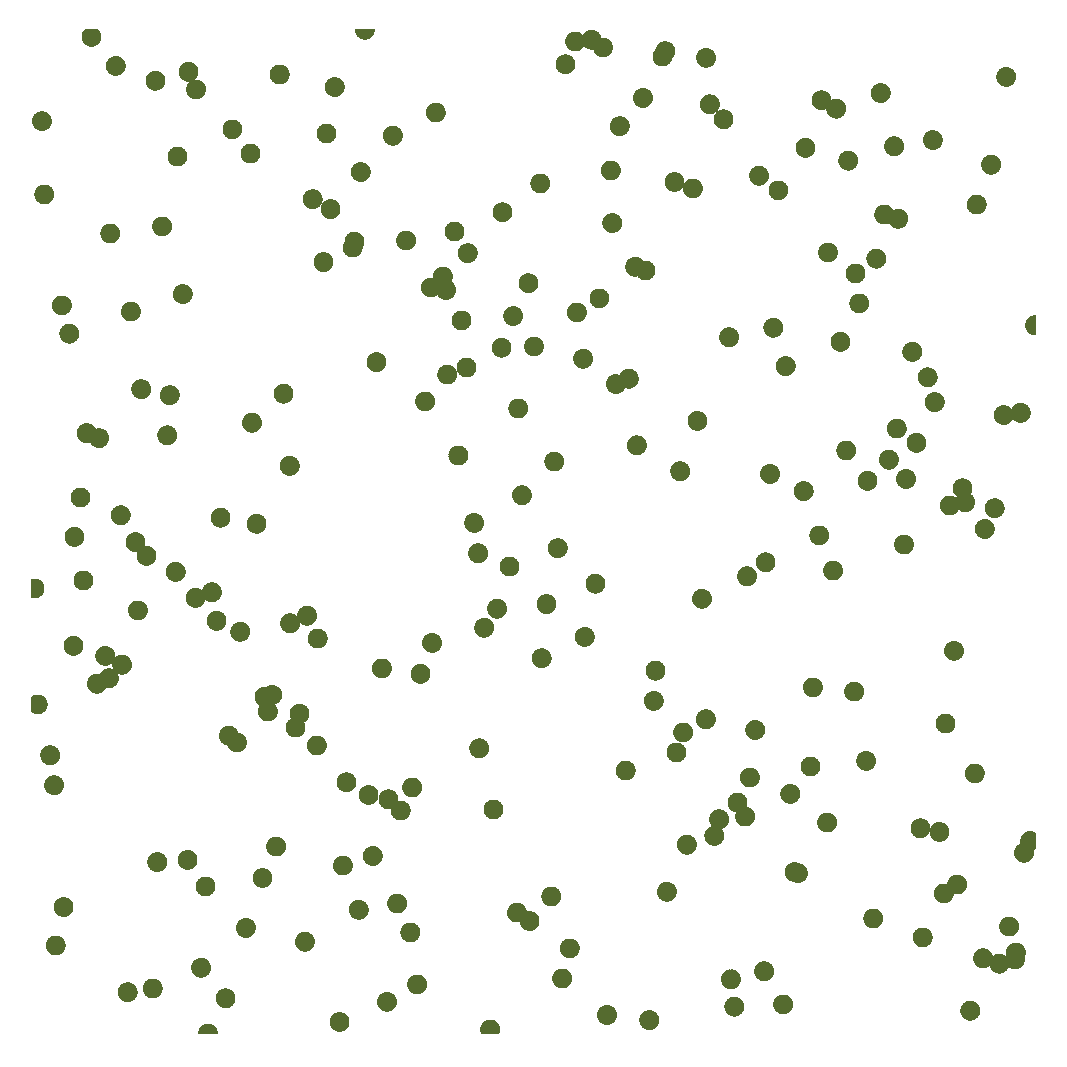
\includegraphics[width=0.2\columnwidth,page=1]{pointset/points-nrooks-n256.pdf}
  };

  \begin{scope}[x={(image.south east)},y={(image.north west)}]
  \draw[black,thick] (0,0) rectangle (1,1);
  \end{scope}
\end{tikzpicture} 
&
\begin{tikzpicture}
  \node[anchor=south west,inner sep=0] (image) at (0,0)
  {
    \pdfliteral{ 1 w}
\includegraphics[width=0.2\columnwidth,page=1]{power-spectra/powerspectrum-nrooks-n4096.png}
  };

  \begin{scope}[x={(image.south east)},y={(image.north west)}]
  \draw[black,thick] (0,0) rectangle (1,1);
  \end{scope}
\end{tikzpicture}
&
\begin{tikzpicture}
  \node[anchor=south west,inner sep=0] (image) at (0,0)
  {
    \pdfliteral{ 1 w}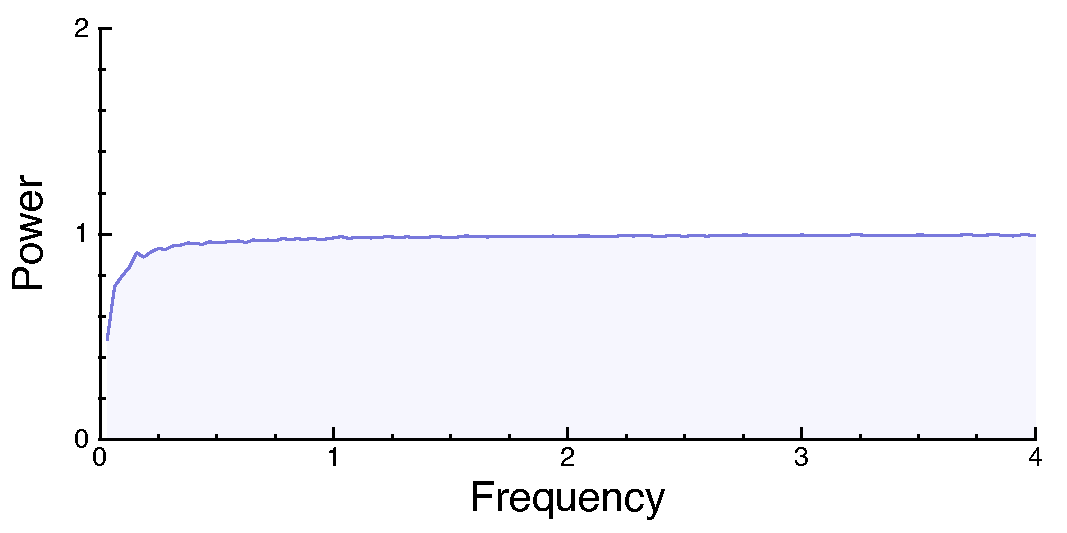
\includegraphics[width=0.4\columnwidth,page=1]{power-spectra/radial-mean-nrooks-n1024.pdf}
  };

  \begin{scope}[x={(image.south east)},y={(image.north west)}]
  \draw[black,thick] (0,0) rectangle (1,1);
  \end{scope}
\end{tikzpicture}\\
%
%==================
%
\rotatebox{90}{\qquad\quad Halton} & 
\begin{tikzpicture}
  \node[anchor=south west,inner sep=0] (image) at (0,0)
  {
    \pdfliteral{ 1 w}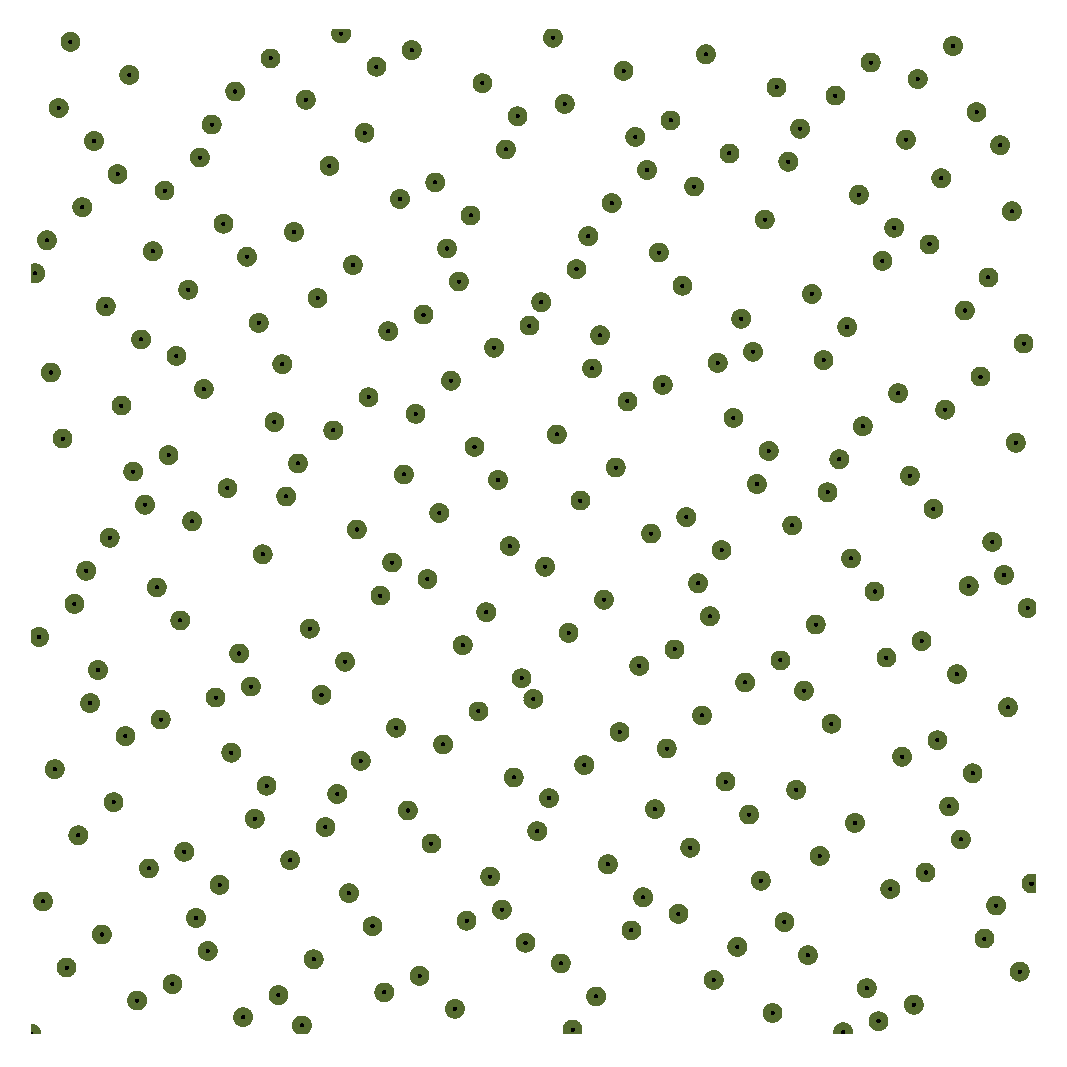
\includegraphics[width=0.2\columnwidth,page=1]{pointset/points-halton-n256.pdf}
  };

  \begin{scope}[x={(image.south east)},y={(image.north west)}]
  \draw[black,thick] (0,0) rectangle (1,1);
  \end{scope}
\end{tikzpicture} 
&
\begin{tikzpicture}
  \node[anchor=south west,inner sep=0] (image) at (0,0)
  {
    \pdfliteral{ 1 w}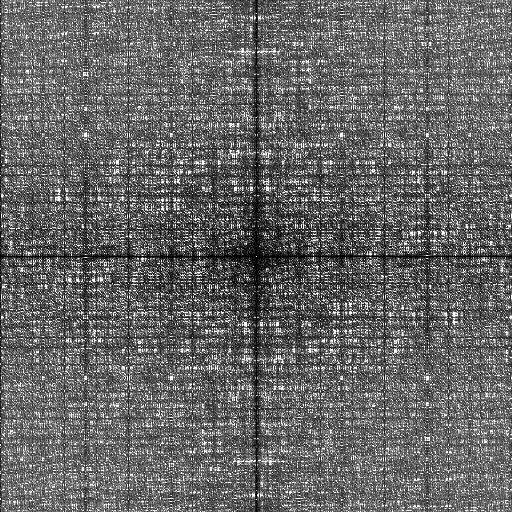
\includegraphics[width=0.2\columnwidth,page=1]{power-spectra/powerspectrum-halton-n4096.png}
  };

  \begin{scope}[x={(image.south east)},y={(image.north west)}]
  \draw[black,thick] (0,0) rectangle (1,1);
  \end{scope}
\end{tikzpicture}
&
\begin{tikzpicture}
  \node[anchor=south west,inner sep=0] (image) at (0,0)
  {
    \pdfliteral{ 1 w}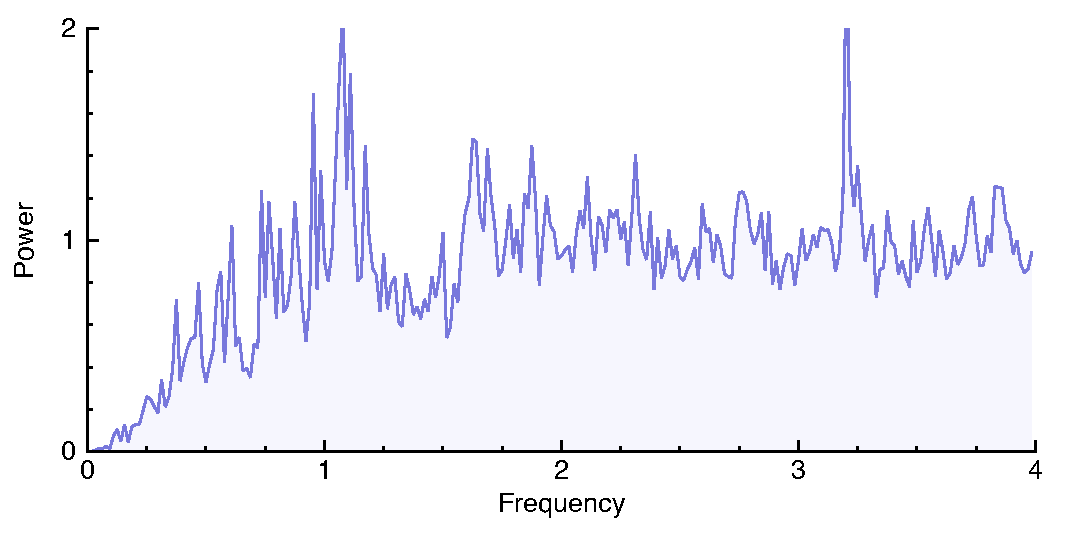
\includegraphics[width=0.4\columnwidth,page=1]{power-spectra/radial-mean-halton-n4096.pdf}
  };

  \begin{scope}[x={(image.south east)},y={(image.north west)}]
  \draw[black,thick] (0,0) rectangle (1,1);
  \end{scope}
\end{tikzpicture}\\
%
%==============
%
\rotatebox{90}{\qquad Hammerslay} & 
\begin{tikzpicture}
  \node[anchor=south west,inner sep=0] (image) at (0,0)
  {
    \pdfliteral{ 1 w}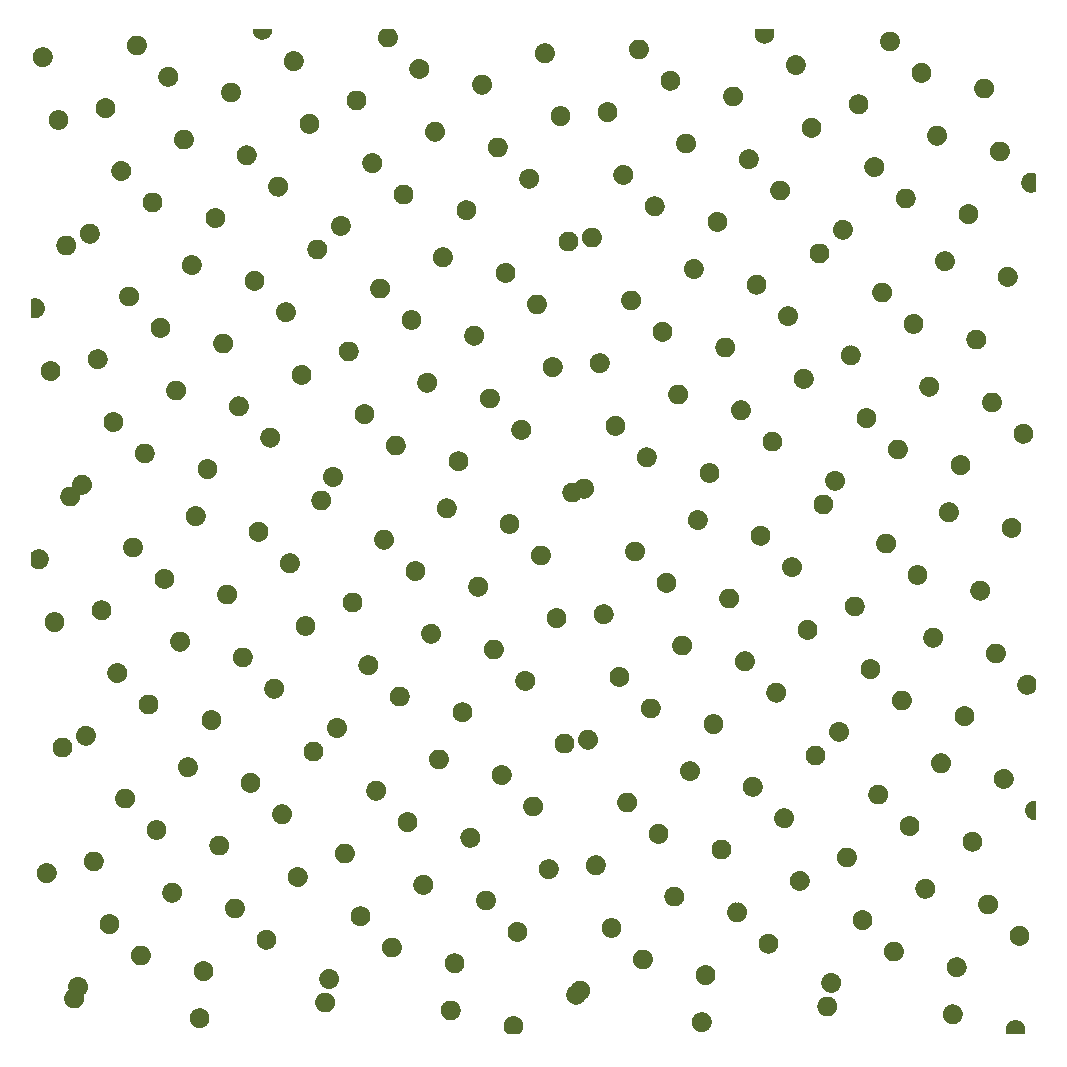
\includegraphics[width=0.2\columnwidth,page=1]{pointset/points-hammerslay-n256.pdf}
  };

  \begin{scope}[x={(image.south east)},y={(image.north west)}]
  \draw[black,thick] (0,0) rectangle (1,1);
  \end{scope}
\end{tikzpicture} 
&
\begin{tikzpicture}
  \node[anchor=south west,inner sep=0] (image) at (0,0)
  {
    \pdfliteral{ 1 w}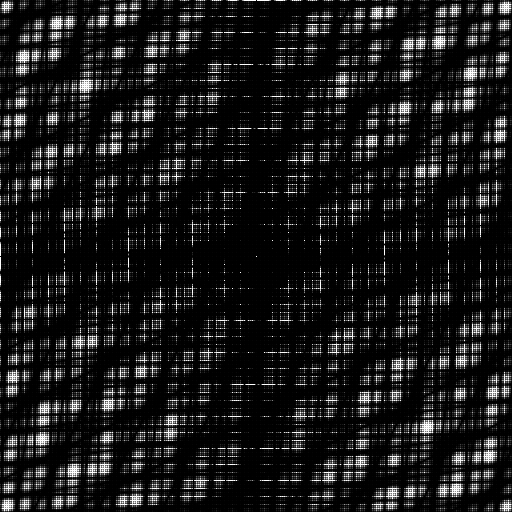
\includegraphics[width=0.2\columnwidth,page=1]{power-spectra/powerspectrum-hammerslay-n4096.png}
  };

  \begin{scope}[x={(image.south east)},y={(image.north west)}]
  \draw[black,thick] (0,0) rectangle (1,1);
  \end{scope}
\end{tikzpicture}
&
\begin{tikzpicture}
  \node[anchor=south west,inner sep=0] (image) at (0,0)
  {
    \pdfliteral{ 1 w}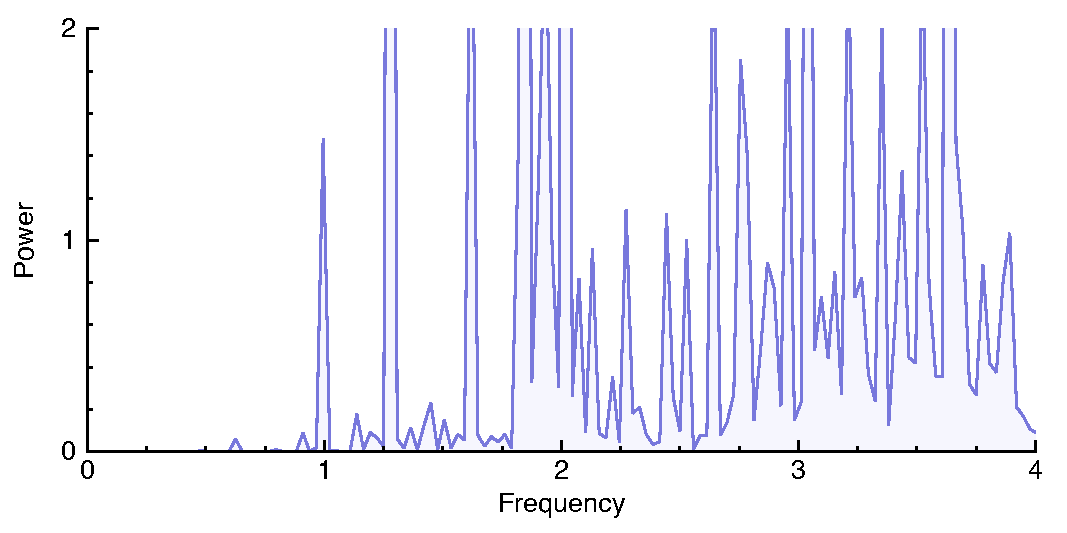
\includegraphics[width=0.4\columnwidth,page=1]{power-spectra/radial-mean-hammerslay-n4096.pdf}
  };

  \begin{scope}[x={(image.south east)},y={(image.north west)}]
  \draw[black,thick] (0,0) rectangle (1,1);
  \end{scope}
\end{tikzpicture}\\
%
%==============
%
\rotatebox{90}{\qquad\quad Regular} & 
\begin{tikzpicture}
  \node[anchor=south west,inner sep=0] (image) at (0,0)
  {
    \pdfliteral{ 1 w}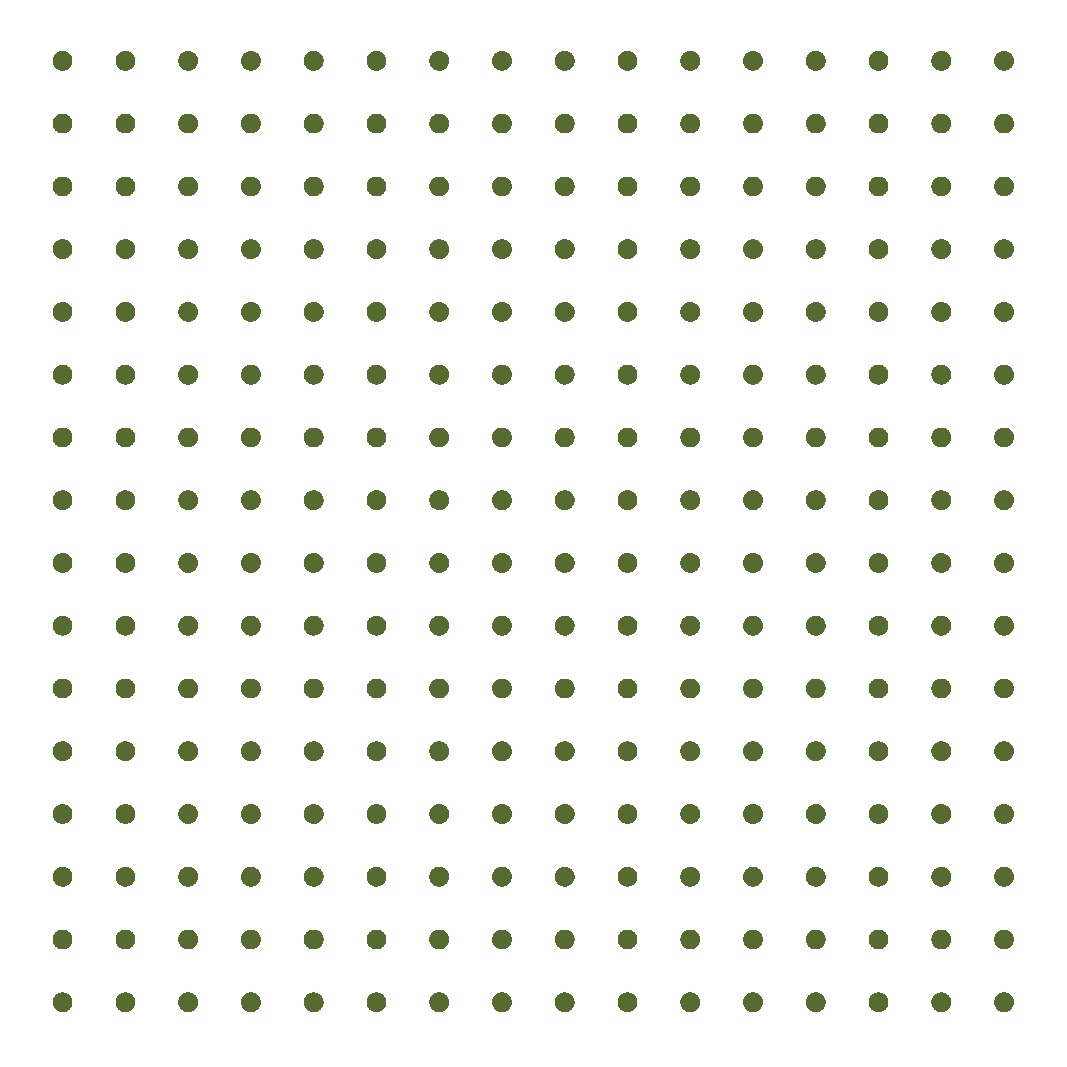
\includegraphics[width=0.2\columnwidth,page=1]{pointset/points-regular-n256.pdf}
  };

  \begin{scope}[x={(image.south east)},y={(image.north west)}]
  \draw[black,thick] (0,0) rectangle (1,1);
  \end{scope}
\end{tikzpicture} 
&
\begin{tikzpicture}
  \node[anchor=south west,inner sep=0] (image) at (0,0)
  {
    \pdfliteral{ 1 w}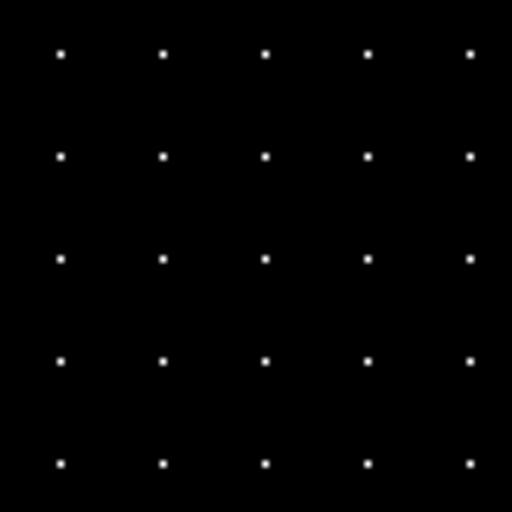
\includegraphics[width=0.2\columnwidth,page=1]{power-spectra/powerspectrum-regular-n256-cropped2.png}
  };

  \begin{scope}[x={(image.south east)},y={(image.north west)}]
  \draw[black,thick] (0,0) rectangle (1,1);
  \end{scope}
\end{tikzpicture}
&
\begin{tikzpicture}
  \node[anchor=south west,inner sep=0] (image) at (0,0)
  {
    \pdfliteral{ 1 w}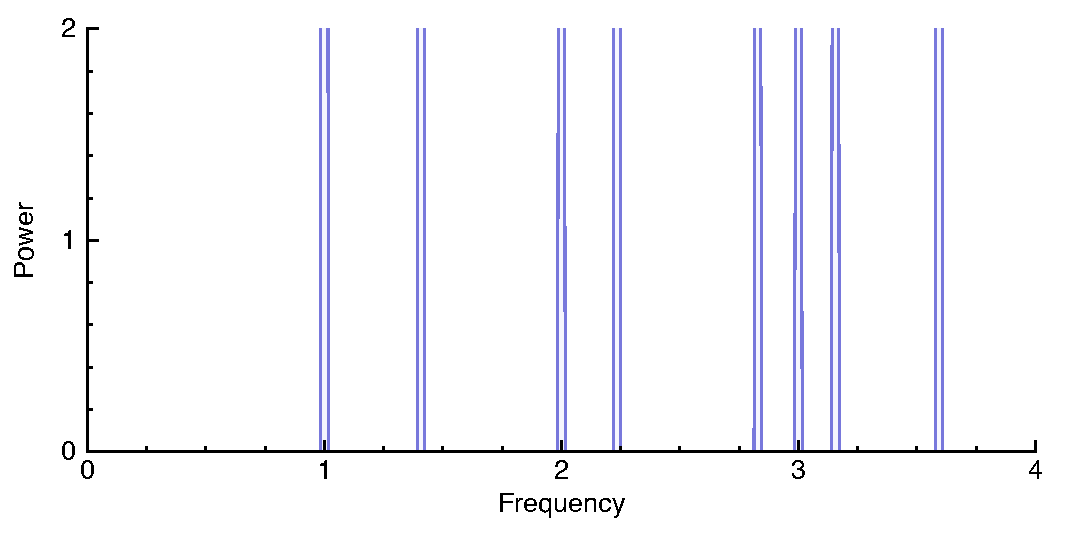
\includegraphics[width=0.4\columnwidth,page=1]{power-spectra/radial-mean-regular-n4096.pdf}
  };

  \begin{scope}[x={(image.south east)},y={(image.north west)}]
  \draw[black,thick] (0,0) rectangle (1,1);
  \end{scope}
\end{tikzpicture}\\
\end{tabular}
%
\caption{\label{fig:points-powspec-radialmean}%
Illustration of some well known sampling patterns with the corresponding Fourier expected power spectra and the corresponding radial mean of their expected power spectra.}
\end{figure}
%

\section{Synthesis of sampling patterns with targeted spectral profiles}

Recently, researchers have noticed the importance of having a \emph{spectral control} on sampling methods. 
The idea behind having a sampler with spectral control is to be able to generate samples %which are guided 
from the pre-assigned Fourier characteristics. Consequently, the samples can spatially arrange themselves according 
to the characteristics assigned in the spectral domain. Parker and colleagues~\cite{Parker:1991:PSHP} were the first to propose an algorithm for manipulating the
power spectra of blue noise halftone patterns. A blue noise spectrum
defined by a step function is used as input to influence the
sample distributions. Recently, Zhou and colleagues~\cite{Zhou:2012} construct point sets matching a Fourier power spectrum function by performing 
a gradient descent optimization on an energy derived from the autocorrelation function. 
Such a Fourier power spectrum function can be either obtained from a known sampling
method, or completely constructed by the user.


% %----------------------------------------------------------------------------------------
% %	CHAPTER 6
% %----------------------------------------------------------------------------------------
% \chapterimage{ch6.pdf} % Chapter heading image
% \chapter{Case studies}
% In this chapter, we will present a suite of tests that may be used to compare the efficacy of sampling patterns when used in numerical integration. We will then tabulate this comparison, identifying the strengths and weaknesses of the different sampling strategies described in chapter~\ref{ch:stateoftheart}. Our test suite will encompass a variety of integrands of various dimensionalities as well as smoothness criteria. We will make our code available to facilitate the comparison of any sampling patterns that may be proposed in the future with methods in our chosen set of algorithms. 
% 
% \section{1D integrands}
% \TBC 
% 
% \subsection{Smooth functions}
% \TBC 
% \subsection{Functions with discontinuities}
% \TBC 
% \section{2D integrands}
% \TBC 
% \subsection{Smooth functions}
% \TBC 
% \subsection{Functions with discontinuities}
% \TBC 
% \subsection{Sub-pixel integration}
% \TBC 
% \section{Rendering test suite}
% \TBC 

% 
% \section{Figure}\index{Figure}
% 
% \begin{figure}[h]
% \centering
\includegraphics[scale=0.5]{placeholder}
% \caption{Figure caption}
% \end{figure}

% \chapter{Example slides}\label{ch:exslides}
% The remaining pages in this document contain representative slides for the content in chapter~\ref{ch:stateoftheart}.
% % % \cleardoublepage
% % \phantomsection
% % \setlength{\columnsep}{0.75cm}
% % \addcontentsline{toc}{chapter}{\textcolor{ocre}{Index}}
% % \printindex
% 
% %----------------------------------------------------------------------------------------
% 
% % \includepdf[pages={40-75}]{../SampleCourseSlides/example-wj.pdf}
% 
% 
%----------------------------------------------------------------------------------------
%	BIBLIOGRAPHY
%----------------------------------------------------------------------------------------
\chapterimage{biblio.pdf} % Chapter heading image

% \chapter*{Bibliography}
% \nocite{*}
% \section*{Books}
% \addcontentsline{toc}{section}{Books}
% \printbibliography[heading=bibempty,type=book]
% \section*{Articles}
% \addcontentsline{toc}{section}{Articles}
% \printbibliography[heading=bibempty]
\bibliographystyle{acm}
\bibliography{bibliography.bib}
\addcontentsline{toc}{chapter}{\textcolor{ocre}{Bibliography}}

%----------------------------------------------------------------------------------------

% \includepdf[pages={40-69}]{../SampleCourseSlides/example-wj.pdf}


\end{document}